\documentclass[10pt,aspectratio=169]{beamer}
\usetheme[
%%% option passed to the outer theme
%    progressstyle=fixedCircCnt,   % fixedCircCnt, movingCircCnt (moving is deault)
  ]{boxes}
  
% If you want to change the colors of the various elements in the theme, edit and uncomment the following lines

% Change the bar colors:
%\setbeamercolor{Feather}{fg=red!20,bg=red}

% Change the color of the structural elements:
%\setbeamercolor{structure}{fg=red}

% Change the frame title text color:
%\setbeamercolor{frametitle}{fg=blue}

% Change the normal text color background:
%\setbeamercolor{normal text}{fg=black,bg=gray!10}

%-------------------------------------------------------
% INCLUDE PACKAGES
%-------------------------------------------------------

\usepackage[utf8]{inputenc}
\usefonttheme[onlymath]{serif}
\usepackage[english]{babel}
\usepackage[T1]{fontenc}
\usepackage{amsmath}
\usepackage{helvet}
\usepackage{multirow}
\usepackage{graphicx}
\usepackage{comment}
\usepackage[absolute,overlay]{textpos}
\usepackage{tabularx}
\usepackage{tikz}
\usetikzlibrary{arrows,automata,positioning}
\usetikzlibrary{shapes.multipart}
\usetikzlibrary{decorations.markings}
\usetikzlibrary{matrix}
\usepackage{marvosym}
\usepackage[marvosym]{tikzsymbols}

%-------------------------------------------------------
% DEFFINING AND REDEFINING COMMANDS
%-------------------------------------------------------

% colored hyperlinks
%\renewcommand*{\Footnotemark}[1]{\NCC@makefnmark{#1}}
\newcommand{\chref}[2]{
  \href{#1}{{\usebeamercolor[bg]{Feather}#2}}
}
\newcommand{\tuple}[1]{{\langle #1 \rangle}}
\newcommand{\pre}{\mathsf{pre}}     % precondition
\newcommand{\eff}{\mathsf{eff}}     % effect
\newcommand{\cond}{\mathsf{cond}}   % conditional effect

\newcommand{\X}{\mathcal{X}}
\newcommand{\F}{\mathcal{F}}
\newcommand{\A}{\mathcal{A}}
\newcommand{\N}{\mathcal{N}}
\newcommand{\I}{\mathcal{I}}
\newcommand{\real}{\mathbb{R}}
\newcommand{\Dw}{\mathcal{D}}
\newcommand{\Xw}{\mathcal{X}}
\newcommand{\Aw}{\mathcal{A}}
\newcommand{\Rw}{\mathcal{R}}
\newcommand{\OO}{\mathcal{O}}
\newcommand{\tOO}{\wt{\OO}}
\newcommand{\II}[1]{\mathbb{I}{\left\{#1\right\}}}
\newcommand{\PP}[1]{\mathbb{P}\left[#1\right]}
\newcommand{\EE}[1]{\mathbb{E}\left[#1\right]}
\newcommand{\EEs}[2]{\mathbb{E}_{#2}\left[#1\right]}
\newcommand{\PPt}[1]{\mathbb{P}_t\left[#1\right]}
\newcommand{\EEt}[1]{\mathbb{E}_t\left[#1\right]}
\newcommand{\PPi}[1]{\mathbb{P}_i\left[#1\right]}
\newcommand{\EEi}[1]{\mathbb{E}_i\left[#1\right]}
\newcommand{\EEp}[1]{\mathbb{E}_{\pi,P}\left[#1\right]}
\newcommand{\EEcp}[2]{\mathbb{E}_{\pi,P}\left[\left.#1\right|#2\right]}
\newcommand{\PPc}[2]{\mathbb{P}\left[#1\left|#2\right.\right]}
\newcommand{\PPct}[2]{\mathbb{P}_t\left[#1\left|#2\right.\right]}
\newcommand{\PPcc}[2]{\mathbb{P}\left[\left.#1\right|#2\right]}
\newcommand{\PPcct}[2]{\mathbb{P}_t\left[\left.#1\right|#2\right]}
\newcommand{\PPcci}[2]{\mathbb{P}_i\left[\left.#1\right|#2\right]}
\newcommand{\EEc}[2]{\mathbb{E}\left[#1\left|#2\right.\right]}
\newcommand{\EEcc}[2]{\mathbb{E}\left[\left.#1\right|#2\right]}
\newcommand{\EEcs}[3]{\mathbb{E}_{#3}\left[\left.#1\right|#2\right]}
\newcommand{\EEcct}[2]{\mathbb{E}_t\left[\left.#1\right|#2\right]}
\newcommand{\EEcci}[2]{\mathbb{E}_i\left[\left.#1\right|#2\right]}
\renewcommand{\th}{\ensuremath{^{\mathrm{th}}}}
\def\argmin{\mathop{\mbox{ arg\,min}}}
\def\argmax{\mathop{\mbox{ arg\,max}}}
\newcommand{\ra}{\rightarrow}

\newcommand{\norm}[1]{\left\|#1\right\|}
\newcommand{\onenorm}[1]{\norm{#1}_1}
\newcommand{\infnorm}[1]{\norm{#1}_\infty}
\newcommand{\iprod}[2]{\left\langle#1,#2\right\rangle}
\newcommand{\ev}[1]{\left\{#1\right\}}
\newcommand{\pa}[1]{\left(#1\right)}
\newcommand{\bpa}[1]{\bigl(#1\bigr)}
\newcommand{\Bpa}[1]{\Bigl(#1\Bigr)}
\newcommand{\sign}{\mbox{sign}}
\newcommand{\wh}{\widehat}
\newcommand{\wt}{\widetilde}
\newcommand{\transpose}{^\top}

\newcommand{\loss}{\ell}
\newcommand{\hloss}{\wh{\loss}}
\newcommand{\hL}{\wh{L}}
\newcommand{\tZ}{\wt{Z}}
\newcommand{\reg}{\mathfrak{R}}
\newcommand{\hreg}{\widehat{\reg}}
\newcommand{\hr}{\wh{r}}
\newcommand{\hv}{\wh{v}}
\newcommand{\hq}{\wh{q}}
\newcommand{\hmu}{\wh{\mu}}
\newcommand{\hR}{\wh{R}}
\newcommand{\tmu}{\wt{\mu}}
\newcommand{\tN}{\wt{N}}
\newcommand{\RE}[2]{\mbox{RE}\left(\left.#1\right\|#2\right)}
\newcommand{\KL}[2]{\mbox{KL}\left(#1\middle\lVert#2\right)}
\newcommand{\DD}[3]{D_{#3}\left(#1\middle\lVert#2\right)}
\newcommand{\DDC}[2]{\DD{#1}{#2}{C}}
\newcommand{\DDS}[2]{\DD{#1}{#2}{S}}

\newcommand{\trho}{\wt{\rho}}

\definecolor{gold}{rgb}{1,0.75,0}
\definecolor{darkred}{rgb}{0.75,0,0}
\setbeamercolor*{goldc}{fg=black,bg=gold}
\definecolor{danrkpurp}{rgb}{0.4,0.2,0.4}
\setbeamercolor*{purpc}{fg=white,bg=darkpurp}
\setbeamercolor*{redc}{fg=white,bg=darkred}
\newcommand{\hG}[1]{\large \textcolor{darkred}{#1}}

\newcommand{\redd}[1]{\textcolor{darkred}{#1}}
\newcommand{\goldd}[1]{\textcolor{gold}{#1}}

\definecolor{ballblue}{rgb}{0.0, 0.5, 0.5}
\definecolor{lightgray}{rgb}{0.85, 0.85, 0.85}

%-------------------------------------------------------
% INFORMATION IN THE TITLE PAGE
%-------------------------------------------------------

\AtBeginSection[]
{
   \begin{frame}
       \frametitle{Session 2A (2nd hour)}
       \tableofcontents[currentsection]
   \end{frame}
}

%-------------------------------------------------------
% THE BODY OF THE PRESENTATION
%-------------------------------------------------------

\begin{document}

%-------------------------------------------------------
% THE TITLEPAGE
%-------------------------------------------------------

\begin{frame}[plain,noframenumbering] % the plain option removes the header from the title page, noframenumbering removes the numbering of this frame only
%  \hspace*{-1cm}
  \begin{tabular}{p{4cm}p{7.5cm}}
	\multicolumn{1}{m{4cm}}{
\includegraphics[height=5cm]{images/w189_709_summer-logo.jpg}} &
	\multicolumn{1}{m{7.5cm}}{\textbf{\Large \color{ballblue} Deep Learning \& Applications} {\Huge \color{white} H} {\large Vicen\c{c} G\'omez \& Anders Jonsson}}
  \end{tabular}
\end{frame}

\setbeamertemplate{frametitle}
{
	\vspace{0.45cm}
    {\hspace{0.4cm} \color{ballblue} \insertframetitle}
}

\addtobeamertemplate{frametitle}{}{%
\begin{tikzpicture}[remember picture,overlay]
\node[anchor=north west,yshift=2pt] at (current page.north west) {
\includegraphics[height=1.4cm]{images/w189_709_summer-logo.jpg}};
\node[anchor=north west,yshift=-1.2cm,xshift=1.4cm,color={rgb:white,3;green,6;blue,5},fill={rgb:white,3;green,6;blue,5}] (rect) at (current page.north west) [draw,minimum width=15cm,minimum height=5pt,inner sep=0pt] {};
%\draw[anchor=north west,color={rgb:white,3;green,6;blue,5},fill={rgb:white,3;green,6;blue,5}] at (current page.north west) (0.5,-0.2) rectangle (11.5,-0.3);
\end{tikzpicture}}

\setbeamertemplate{footline}[text line]{%
  \parbox{\linewidth}{\vspace*{-8pt}\hspace*{5.3cm}\insertpagenumber\hfill www.barcelonagse.eu}}
\setbeamertemplate{navigation symbols}{}

\begin{frame}
    \frametitle{Session 2A: Latent variable models}
    \tableofcontents
\end{frame}

\section{Introduction}

%\begin{frame}
%  \frametitle{Supervised learning}
%  \begin{itemize}
%	\item Input set $\mathcal{X}$
%	\item Output set $\mathcal{Y}$ (yes/no, real number, probability)
%	\item {\color{red} Unknown target function} $f:\mathcal{X}\rightarrow \mathcal{Y}$
%	\item {\color{blue} Training set} $S=\{(x_1,y_1),\ldots,(x_N,y_N)\}$ s.t.~$\forall i$, $f(x_i)=y_i$
%	\item {\color{green} Hypothesis set} $\mathcal{H}=\{h_1,\ldots,h_m\}$, where each $h_j:\mathcal{X}\rightarrow \mathcal{Y}$ is a possible estimation of $f$
%	\item {\color{cyan} Final hypothesis} $g\in\mathcal{H}$: hypothesis in $\mathcal{H}$ that approximates $f$, selected by learning algorithm $\mathcal{A}$ on training set $S$
% \end{itemize}
%\end{frame}


\begin{frame}
  \frametitle{Learning Problems}
\begin{center}
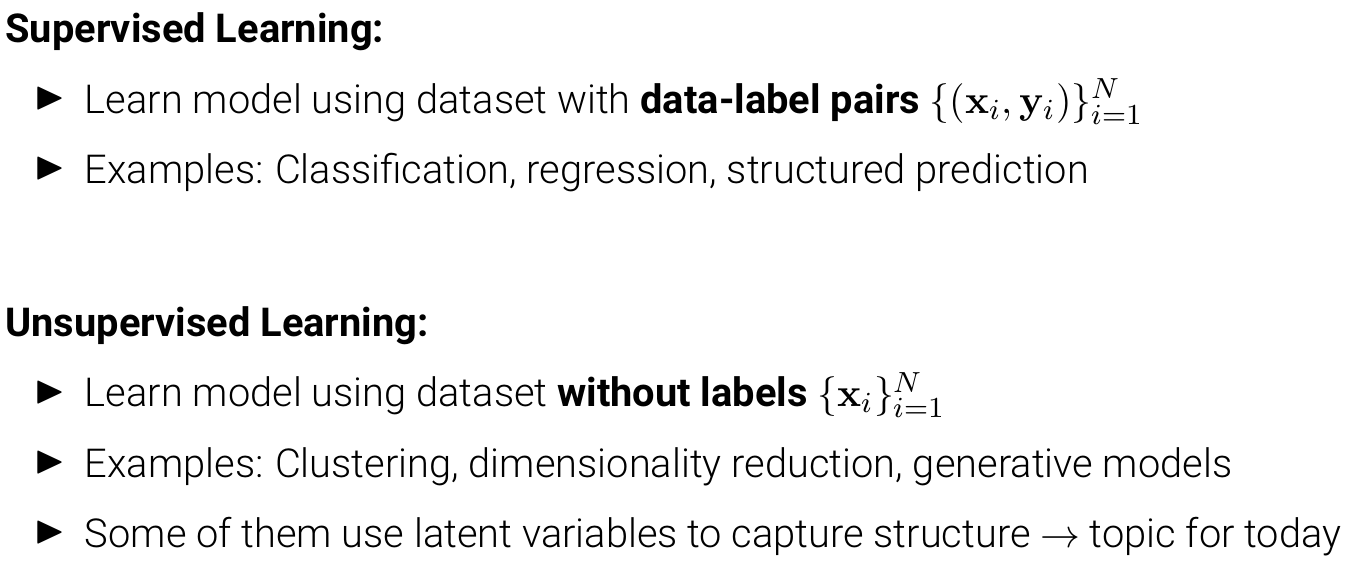
\includegraphics[width=.9\textwidth]{images/s1}
\end{center}

\end{frame}


\begin{frame}
  \frametitle{Latent Variable Models}
\begin{center}
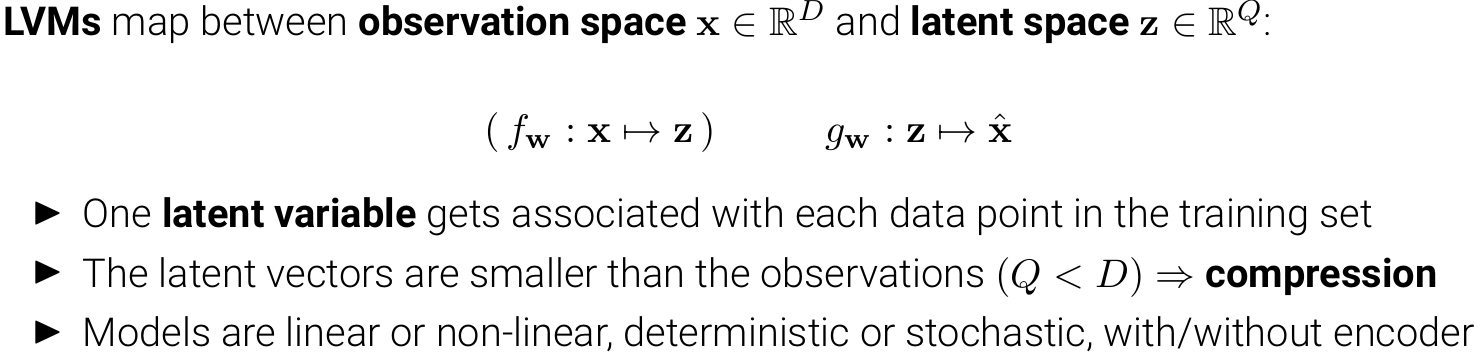
\includegraphics[width=.9\textwidth]{images/s2}
\end{center}


\small{\textbf{A little taxonomy}:}
\begin{center}
\small{\begin{tabular}{|c|c|c|}
\hline & \emph{Deterministic} & \emph{Probabilistic} \\
\hline \emph{Linear} & Principal Component Analysis & Probabilistic PCA\\
\hline $\begin{array}{c}\text{\emph{Nonlinear, Noninvertible}}\end{array}$
 & \textbf{Deep Autoencoder} & \textbf{Variational Autoencoder}\\
\hline $\begin{array}{c}\text{\emph{Nonlinear, Invertible}}\end{array}$ & & \textbf{Normalizing flows}\\\hline
\end{tabular}
}
\end{center}
\end{frame}


\begin{frame}
  \frametitle{Autoencoders}
\begin{center}
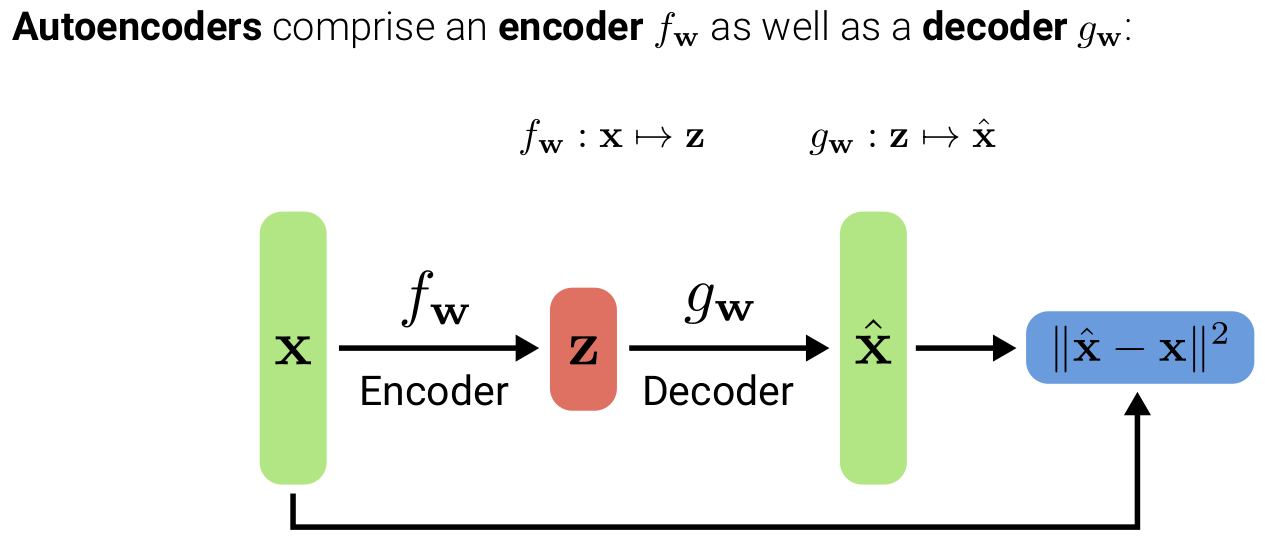
\includegraphics[width=.9\textwidth]{images/s3}
\end{center}
\begin{itemize}
\item Models of this type are called \textbf{autoencoders} as they predict their input as output
\end{itemize}

\end{frame}

\begin{frame}
  \frametitle{Autoencoders}
\begin{center}
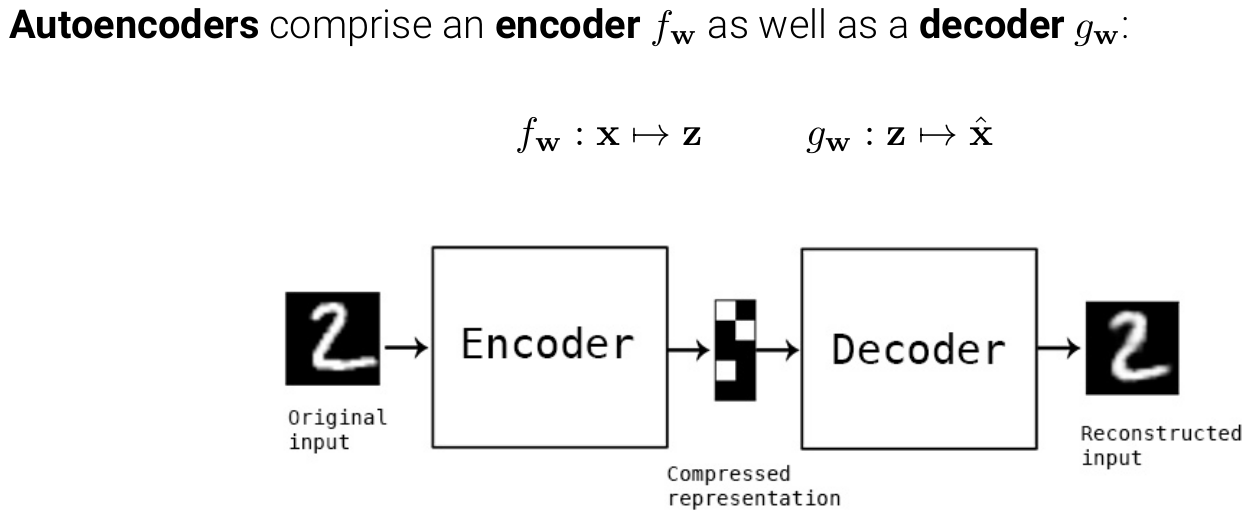
\includegraphics[width=.9\textwidth]{images/s4}
\end{center}
\begin{itemize}
\item Models of this type are called \textbf{autoencoders} as they predict their input as output
\end{itemize}
\end{frame}



\begin{frame}
  \frametitle{Generative Models}
\small{
\begin{itemize}[<+->]
\item Generative modeling is a broad area of ML which deals with models of 
\textbf{probability distributions} $p(\mathbf{x})$ over data points $\mathbf{x}$
\item The generative model's task is to capture dependencies / structural regularities in the data
\item \textbf{Generative latent variable models} capture the structure in the \textbf{latent variables}
\item Intuitively, we are trying to establish a \textbf{theory} for what we observe
\item Some generative models (normalizing flows) allow for computing $p(\mathbf{x})$
\item Others (VAEs) only approximate $p(\mathbf{x})$
\item All generative latent variable models allow to draw samples from $p(\mathbf{x})$
\end{itemize}

}
\end{frame}


\begin{frame}
  \frametitle{Generative Latent Variable Models}
\begin{center}
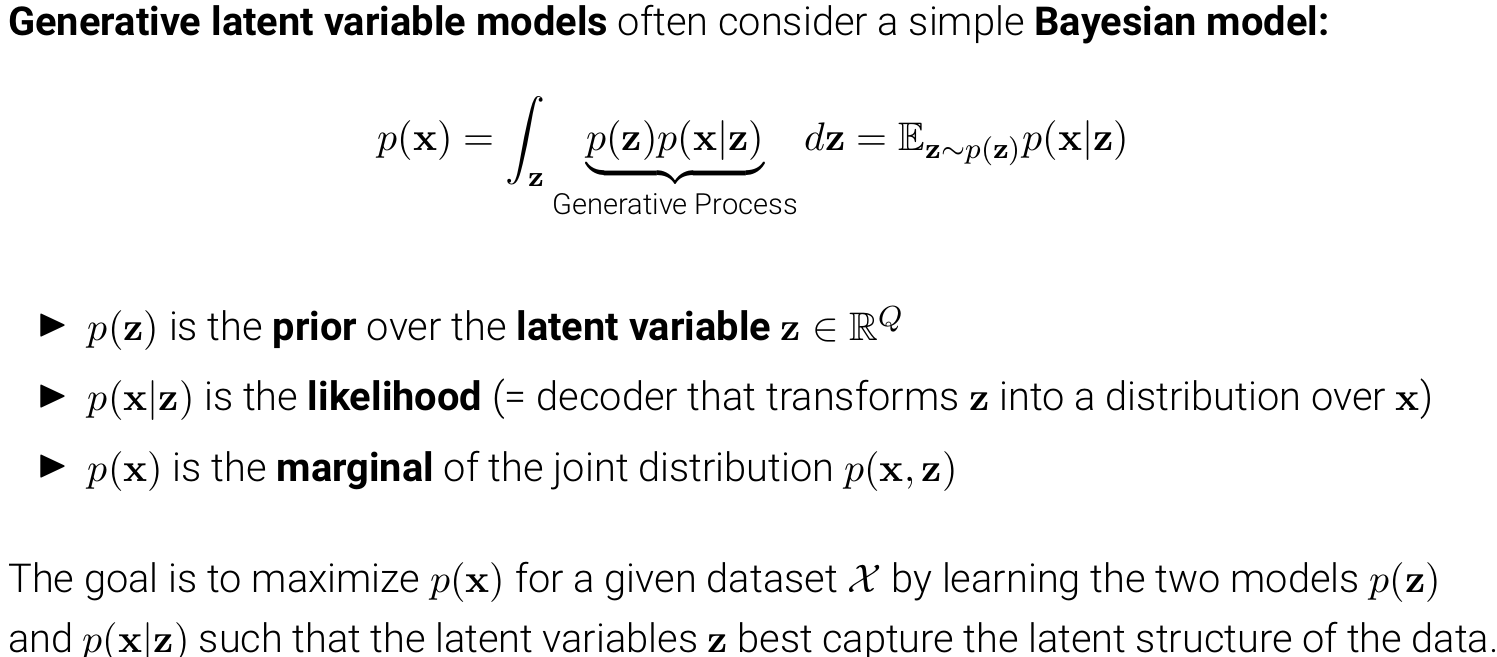
\includegraphics[width=.9\textwidth]{images/s5}
\end{center}
\end{frame}


\begin{frame}
  \frametitle{Generative Latent Variable Models}
\begin{center}
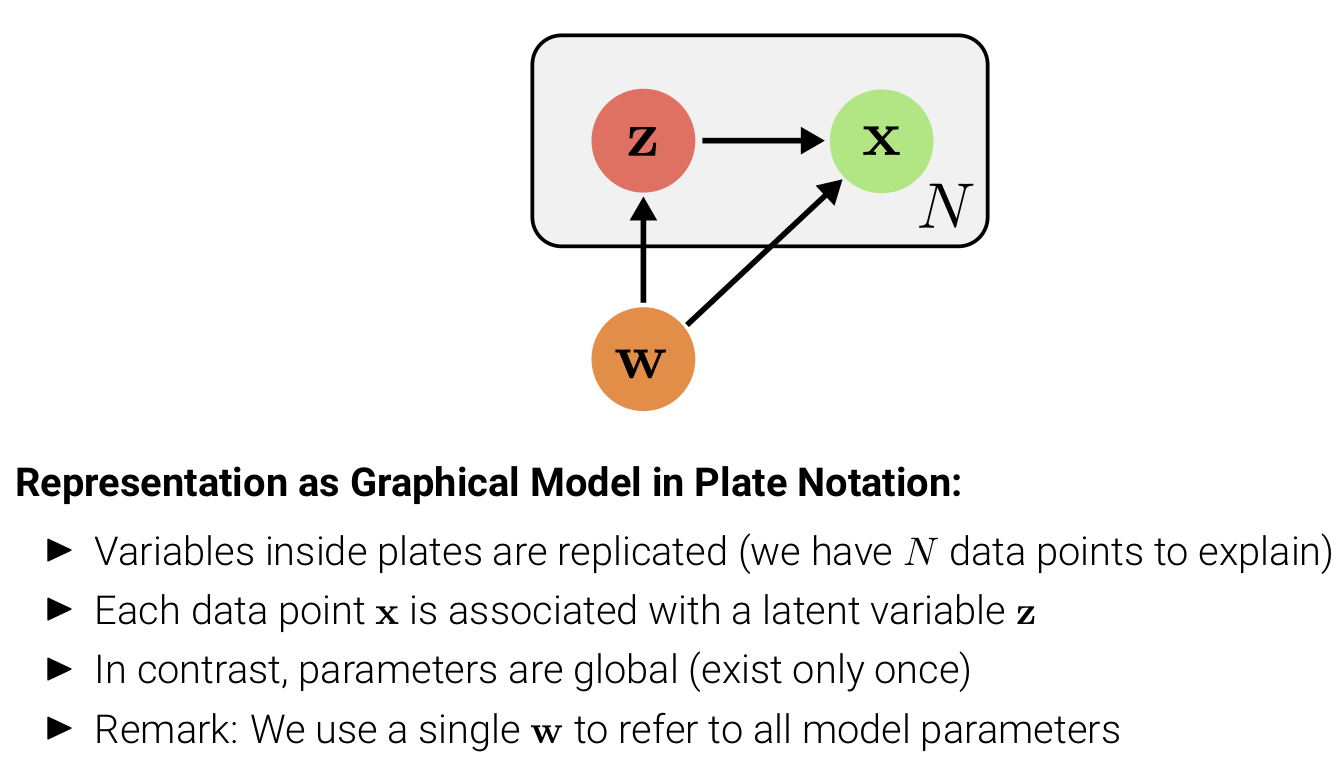
\includegraphics[width=.8\textwidth]{images/s6}
\end{center}
\end{frame}



\begin{frame}
  \frametitle{Example: 1D Manifold in 2D Space}
\begin{center}
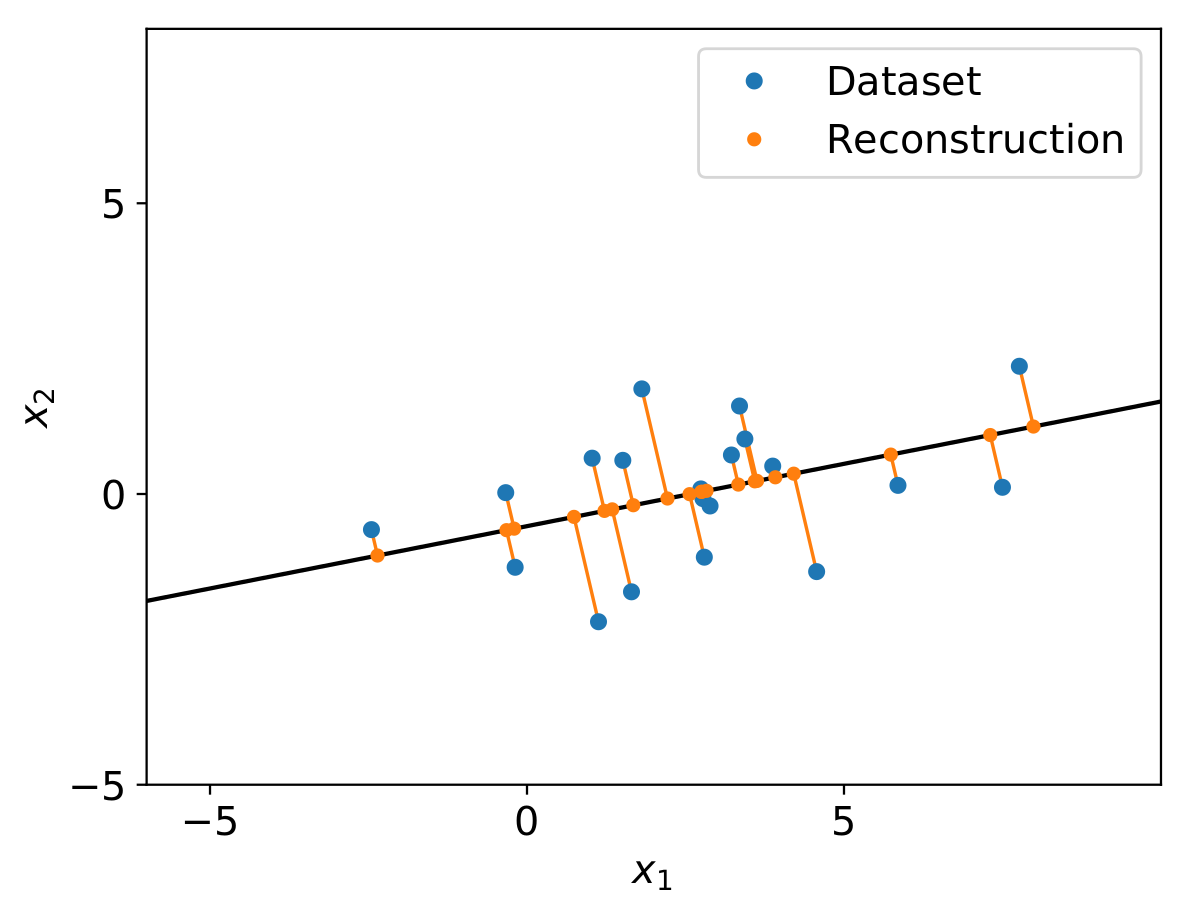
\includegraphics[width=.5\textwidth]{images/s7}
\end{center}
{\color{blue}Original data} $\mathbf{x}$, {\color{orange}Reconstruction} $\hat{\mathbf{x}}$

\end{frame}


\begin{frame}
  \frametitle{Example: Natural Image Manifolds}
\begin{center}
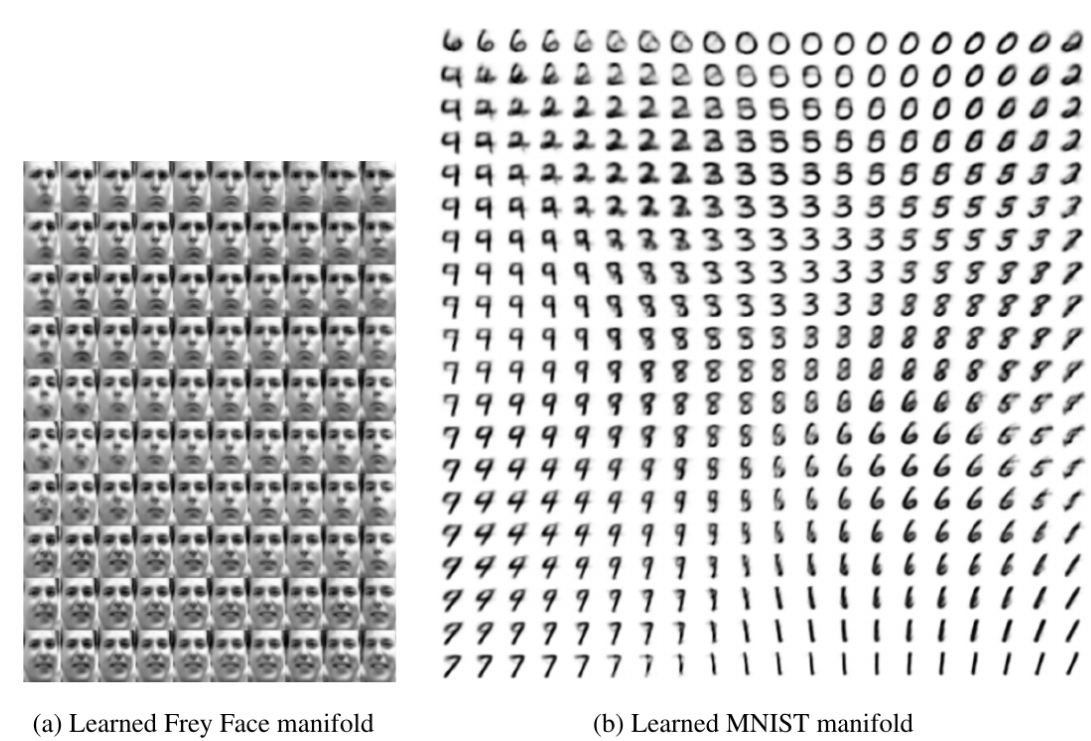
\includegraphics[width=.6\textwidth]{images/s8}
\end{center}
{\small{
\begin{itemize}
\item Visualizing the latent space gives insights into the learned semantics
\end{itemize}
}}
\end{frame}



\section{Autoencoders}


\begin{frame}
  \frametitle{Preliminaries}
\small{
\begin{itemize}[<+->]
\item Let $\mathbf{X}=(\mathbf{x}_1,\hdots,\mathbf{x}_N)^\top\in\mathbb{R}^{N\times D}$ be a dataset of observations $\mathbf{x}_i\in\mathbb{R}^D$
\item Let $\mathbf{Z}=(\mathbf{z}_1,\hdots,\mathbf{z}_N)^\top\in\mathbb{R}^{N\times Q}$ be corresponding latent vars $\mathbf{z}_i\in\mathbb{R}^Q$
\item While $\mathbf{X}$ is observed, $\mathbf{Z}$ is unobserved and needs to be inferred
\item Typically, $Q<D$, i.e., we want to obtain a \textbf{compressed} representation
\item Goal: learn a \textbf{bidirectional mapping} $\mathcal{Z}\leftrightarrow\mathcal{X}$ such that
as much information of $\mathcal{X}$ as possible is retained in $\mathcal{Z}$
\item In other words, encode $\mathbf{x}\rightarrow\mathbf{x}$ such that decoding
$\mathbf{z}\rightarrow\hat{\mathbf{x}}$, leads to a good approximationg of the
original $\mathbf{x}$
\item Simplest autoencoder: a \textbf{linear} bidirectional mapping $\rightarrow$ Principal Component Analysis (\textbf{PCA}) 
\end{itemize}
}
%\begin{center}
%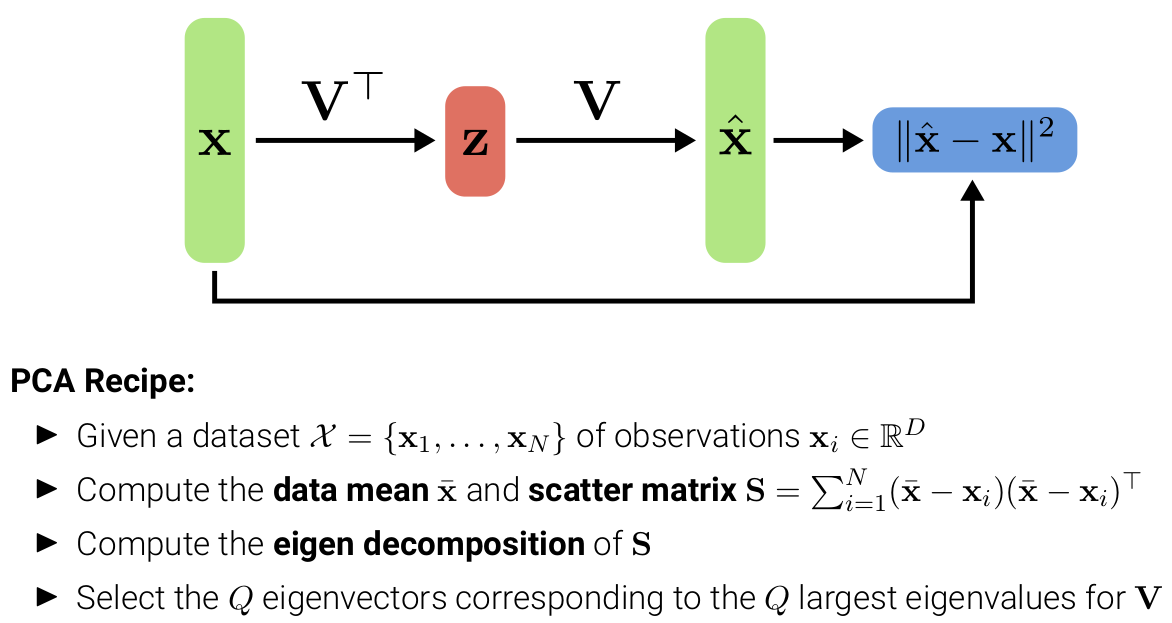
\includegraphics[width=\textwidth]{images/s9}
%\end{center}
\end{frame}

\begin{frame}
  \frametitle{Principal Component Analysis}
\begin{itemize}
\item Principal Component Analysis (PCA) reconstructs the input using a linear model 
\end{itemize}
\begin{center}
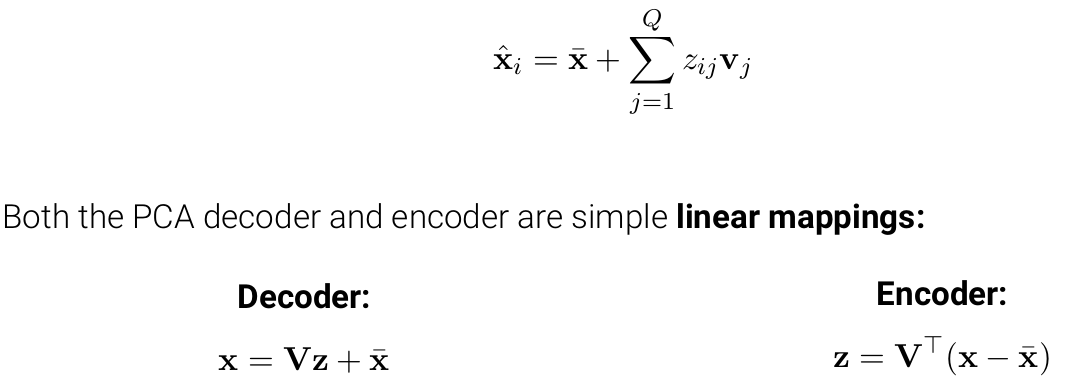
\includegraphics[width=.9\textwidth]{images/s10}
\end{center}
\end{frame}

\begin{frame}
  \frametitle{Principal Component Analysis}
\begin{center}
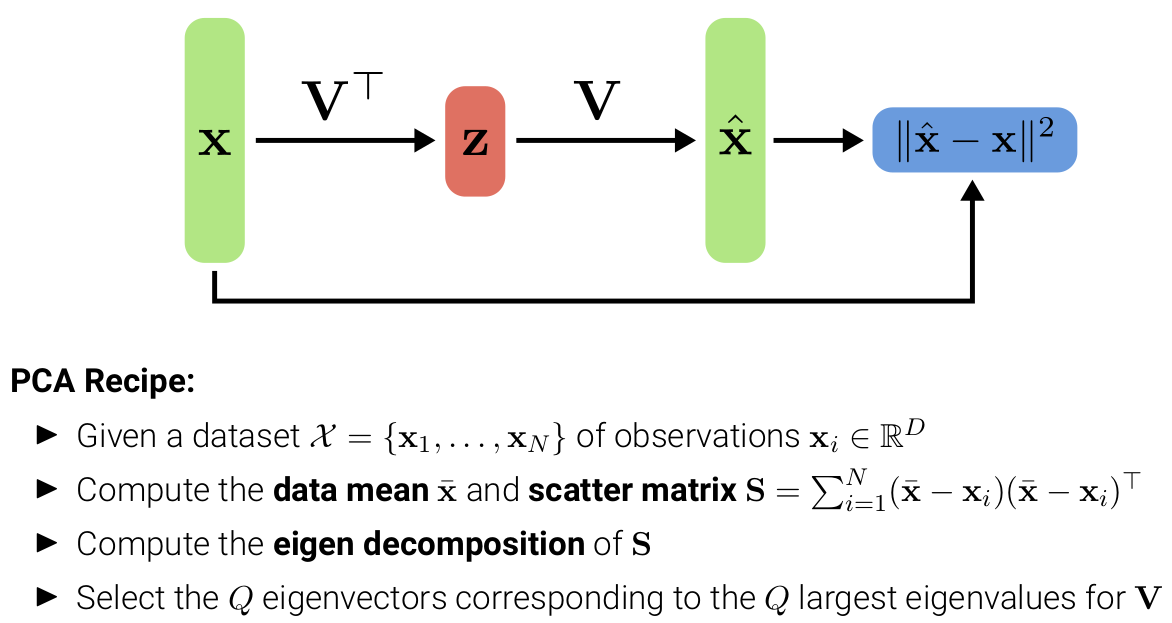
\includegraphics[width=.9\textwidth]{images/s9}
\end{center}
\end{frame}


\begin{frame}
  \frametitle{Results in Synthetic 2D Dataset}
\begin{center}
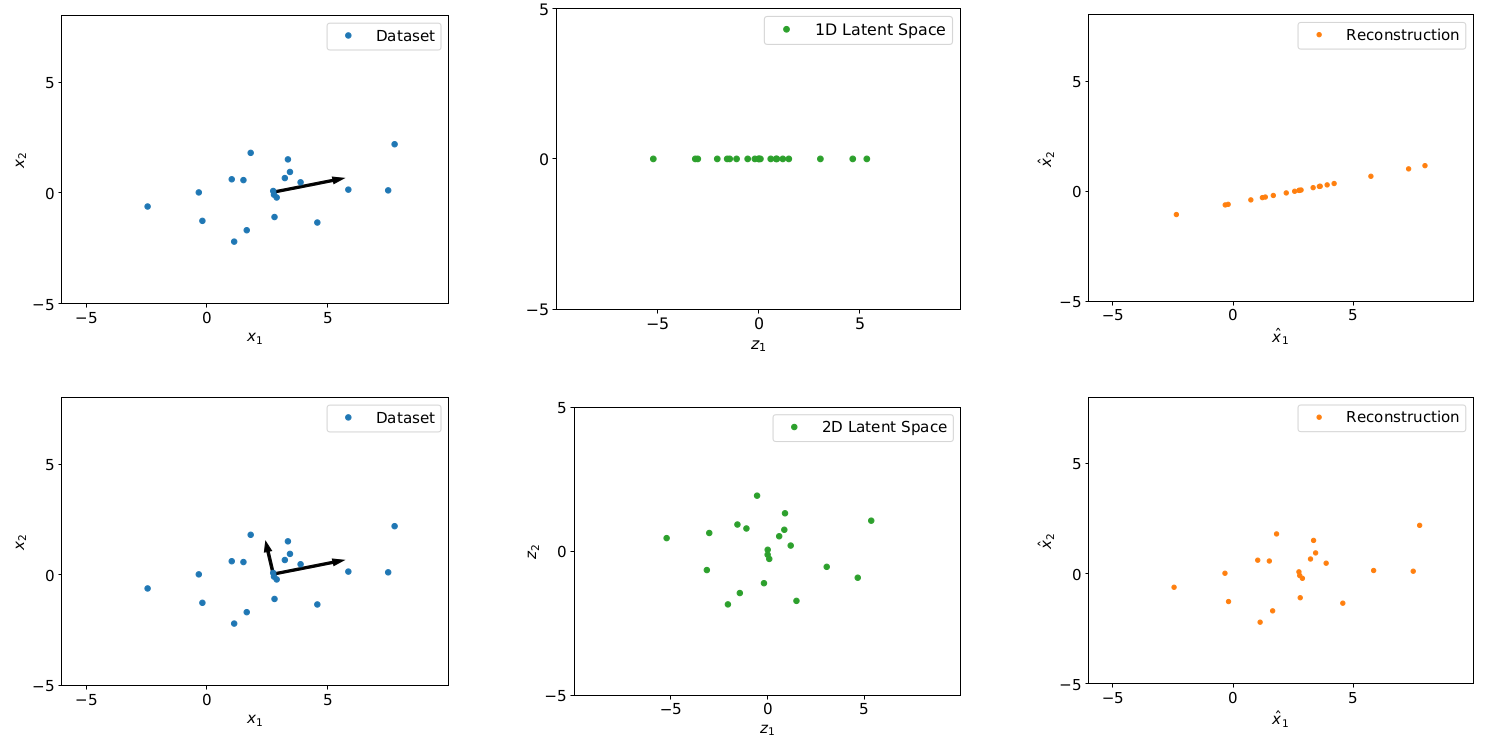
\includegraphics[width=.95\textwidth]{images/s11}
\end{center}
\end{frame}


\begin{frame}
  \frametitle{Results on MNIST}
\begin{center}
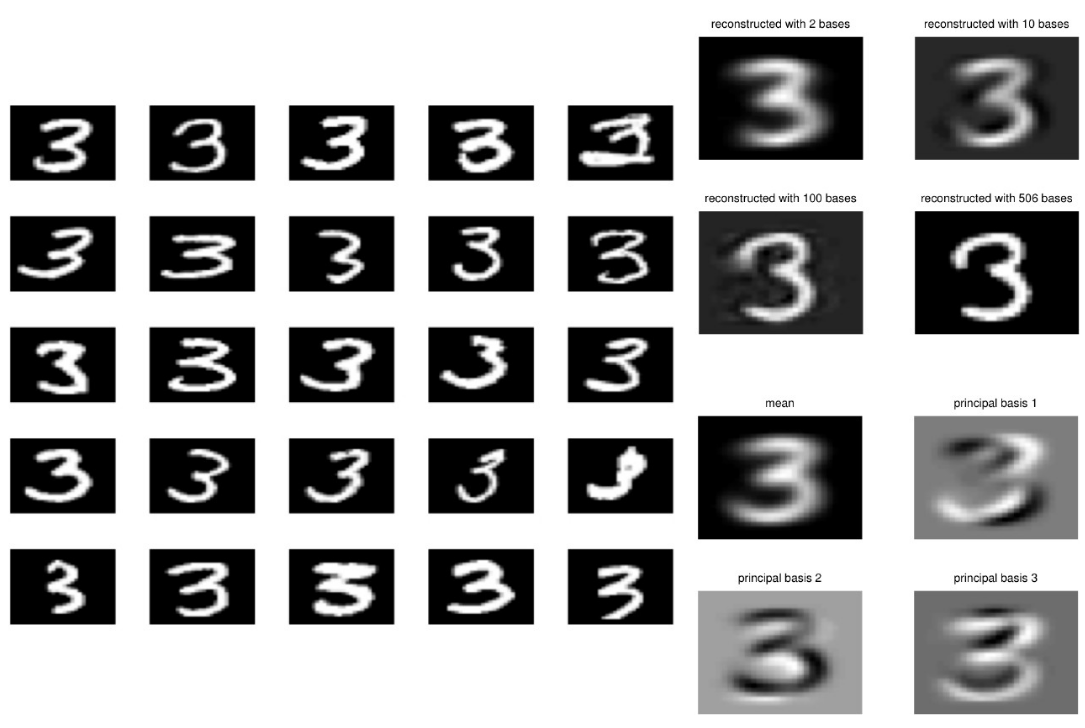
\includegraphics[width=.7\textwidth]{images/s12}
\end{center}
\end{frame}



\begin{frame}
  \frametitle{Results on Faces}
\begin{center}
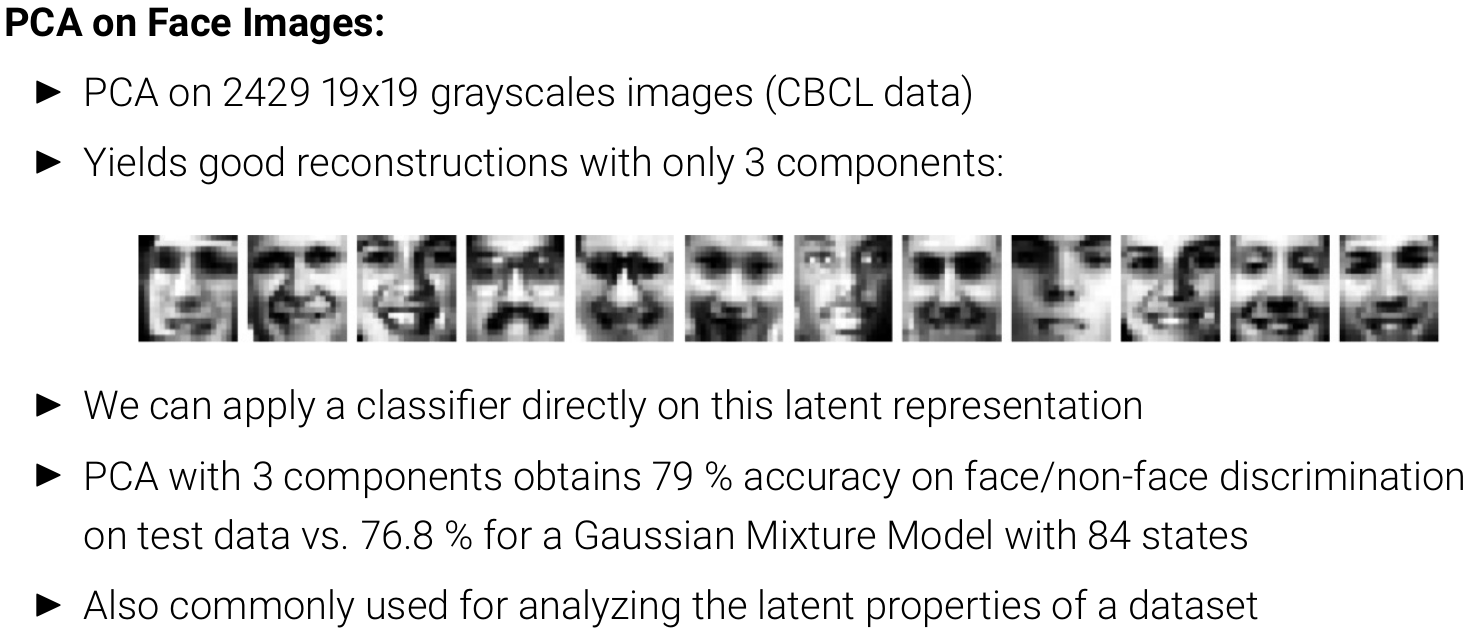
\includegraphics[width=.9\textwidth]{images/s13}
\end{center}
\scriptsize{Turk and Pentland: Face recognition using eigenfaces. CVPR, 1991.}
\end{frame}

\begin{frame}
  \frametitle{Learned Basis (Eigenfaces)}
\begin{center}
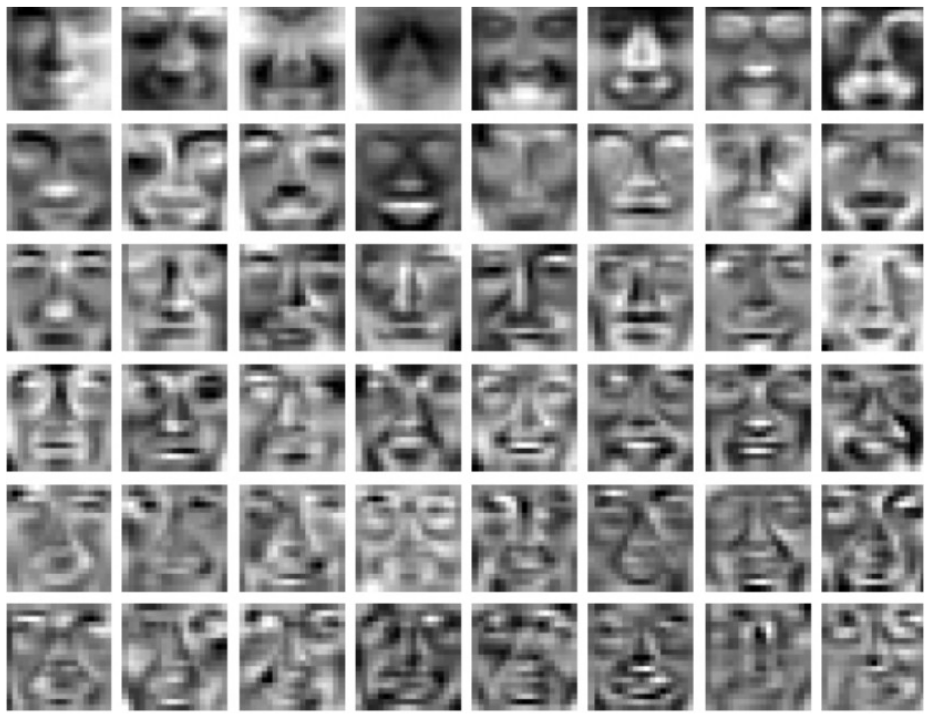
\includegraphics[width=.55\textwidth]{images/s14}
\end{center}
\scriptsize{Turk and Pentland: Face recognition using eigenfaces. CVPR, 1991.}
\end{frame}


\begin{frame}
  \frametitle{Deep Autoencoders}
\begin{center}
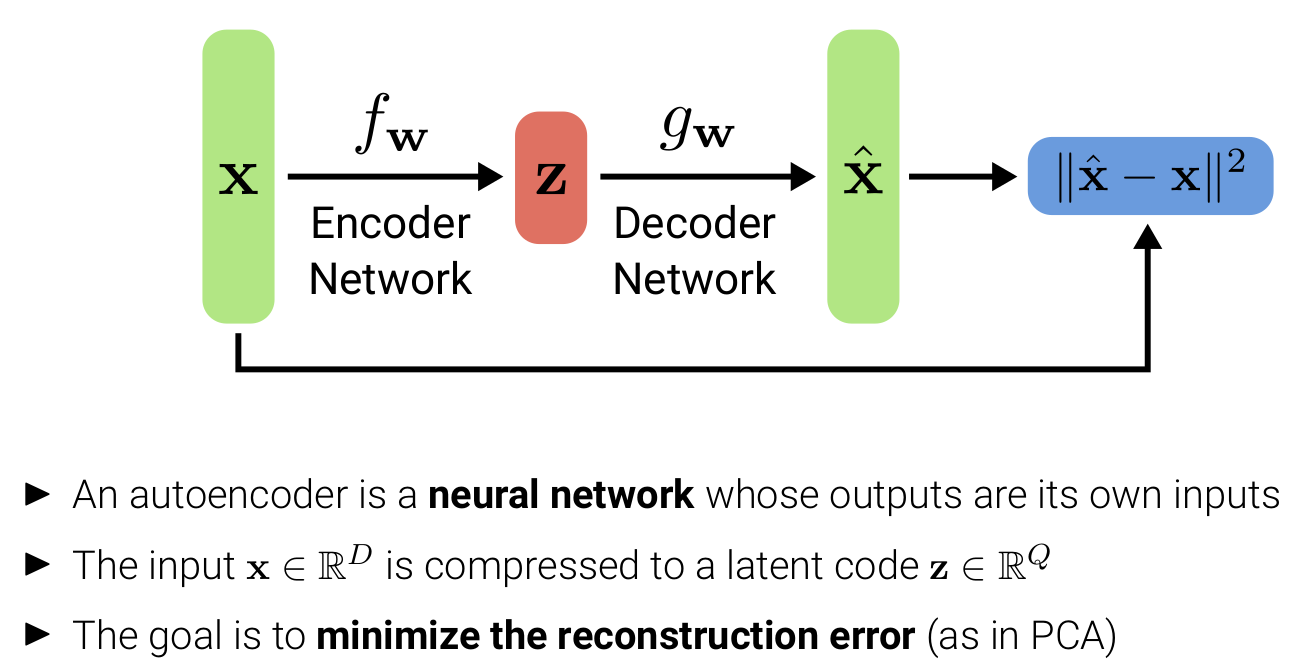
\includegraphics[width=.8\textwidth]{images/s15}
\end{center}
\end{frame}

\begin{frame}
  \frametitle{PCA as special case of Autoencoders}
\begin{center}
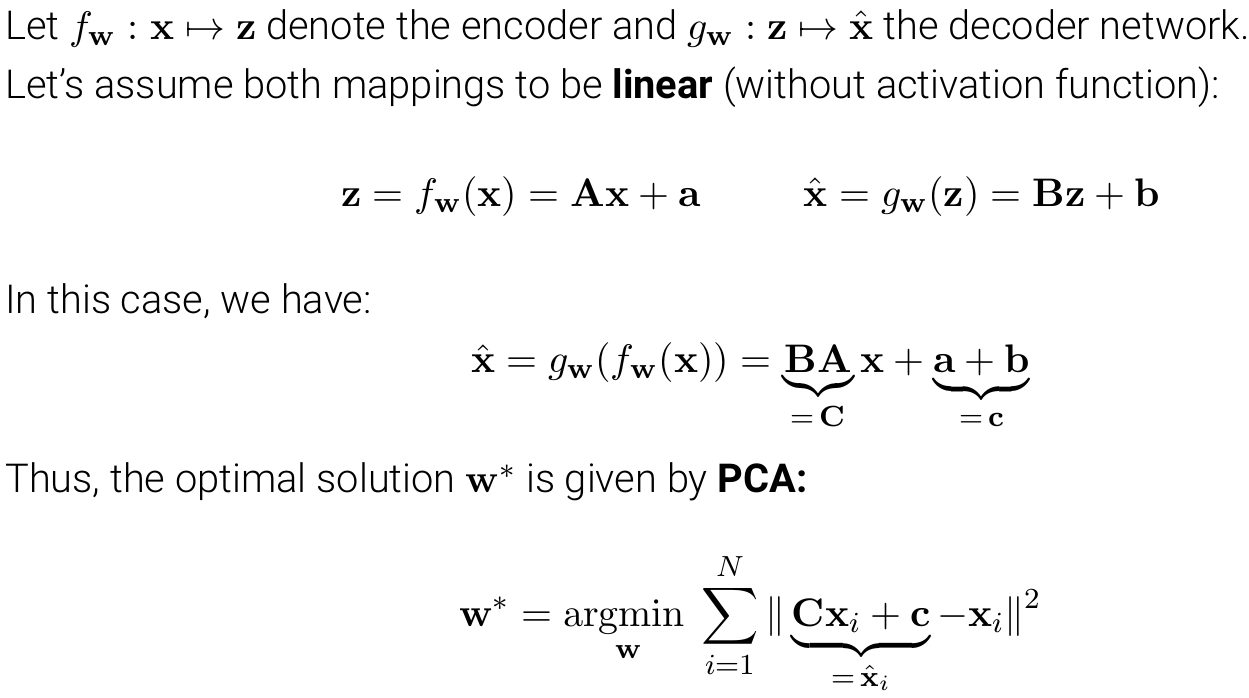
\includegraphics[width=.8\textwidth]{images/s16}
\end{center}
\end{frame}

\begin{frame}
  \frametitle{Results on Synthetic 2D Dataset}
\begin{center}
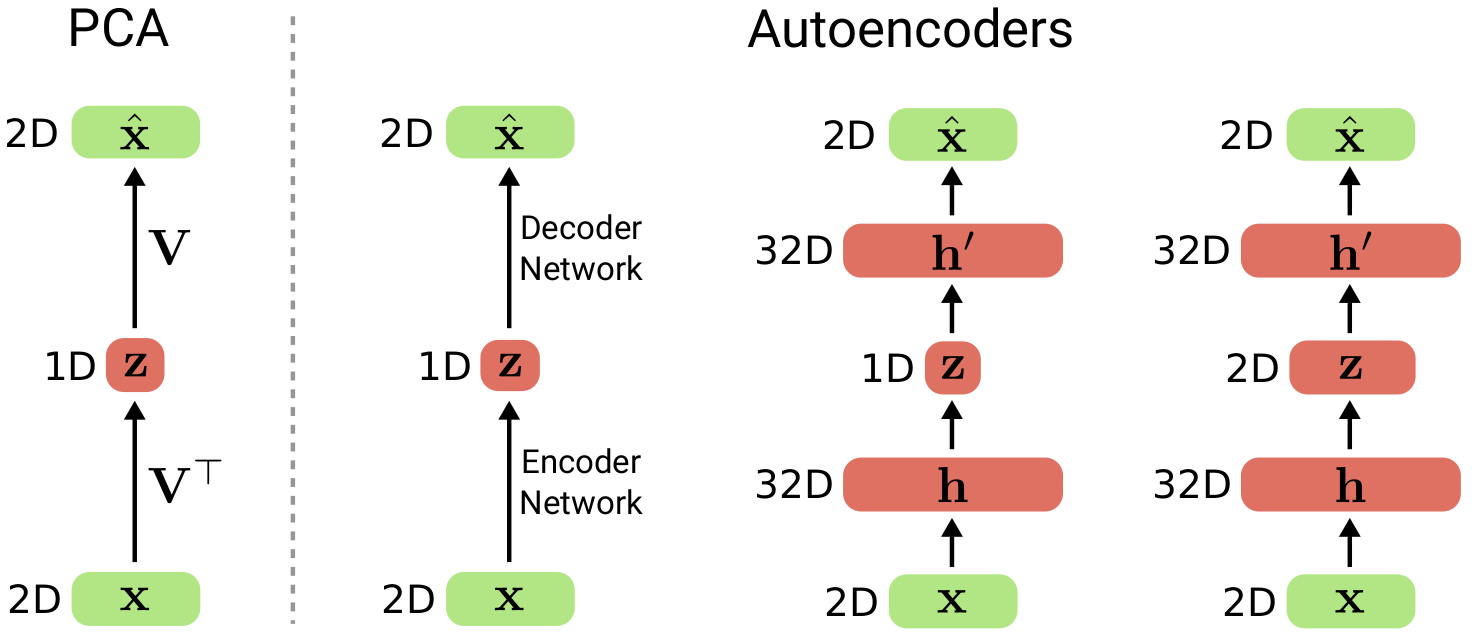
\includegraphics[width=.8\textwidth]{images/s17}
\end{center}
\end{frame}


\begin{frame}
  \frametitle{Results on Synthetic 2D Dataset}
\begin{center}
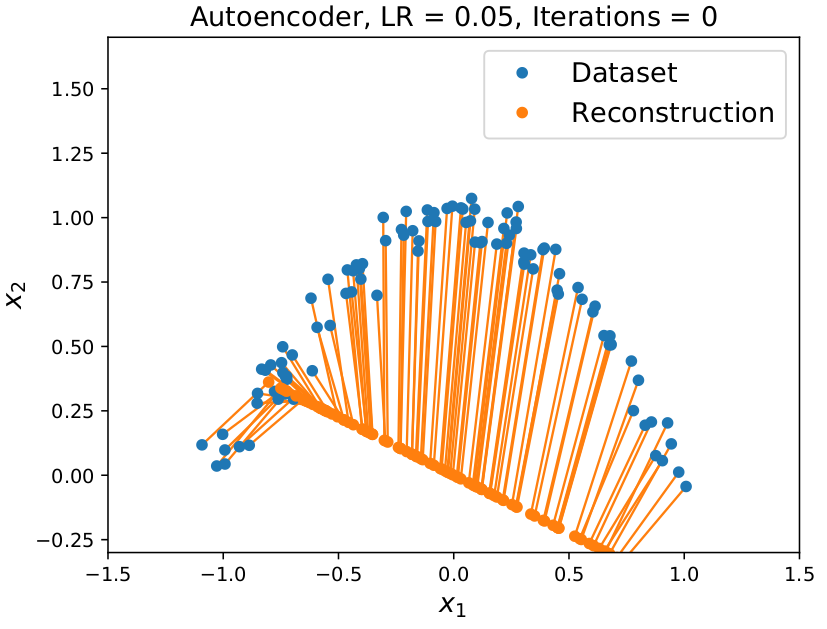
\includegraphics[width=.5\textwidth]{images/s18}
\end{center}
\small{
\begin{itemize}
\item \textbf{Autoencoder reconstruction} with one linear enc/dec layer ($Q=1$)
\end{itemize}
}
\end{frame}

\begin{frame}
  \frametitle{Results on Synthetic 2D Dataset}
\begin{center}
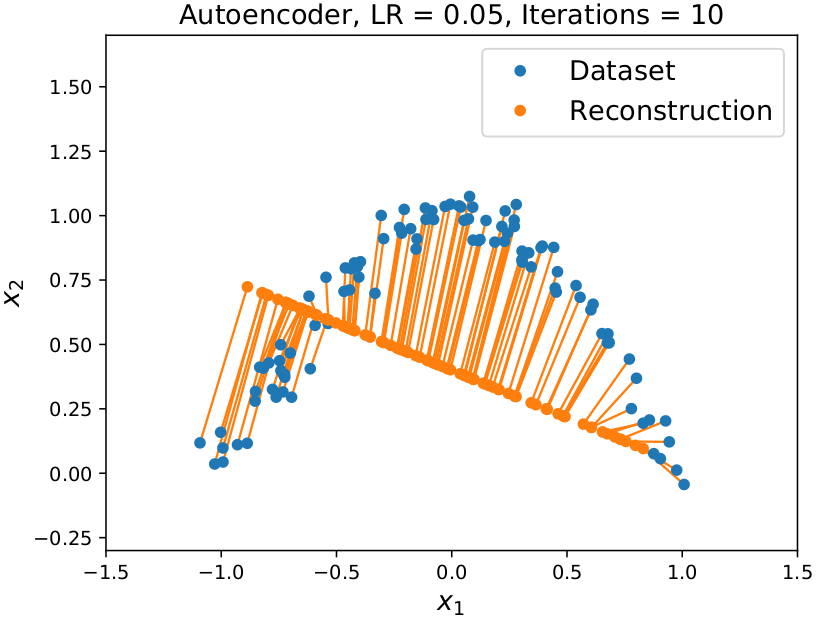
\includegraphics[width=.5\textwidth]{images/s19}
\end{center}
\small{
\begin{itemize}
\item \textbf{Autoencoder reconstruction} with one linear enc/dec layer ($Q=1$)
\end{itemize}
}

\end{frame}
\begin{frame}
  \frametitle{Results on Synthetic 2D Dataset}
\begin{center}
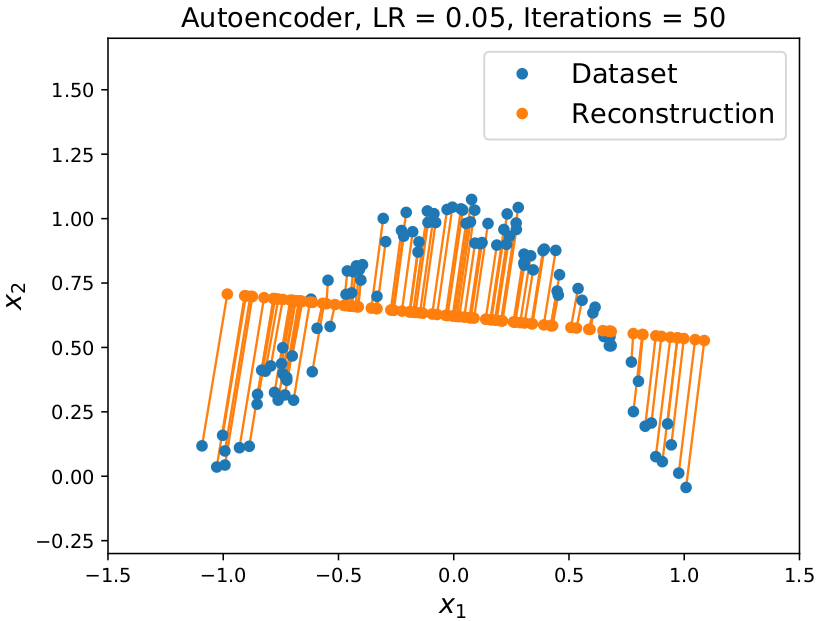
\includegraphics[width=.5\textwidth]{images/s20}
\end{center}
\small{
\begin{itemize}
\item \textbf{Autoencoder reconstruction} with one linear enc/dec layer ($Q=1$)
\end{itemize}
}
\end{frame}

\begin{frame}
  \frametitle{Results on Synthetic 2D Dataset}
\begin{center}
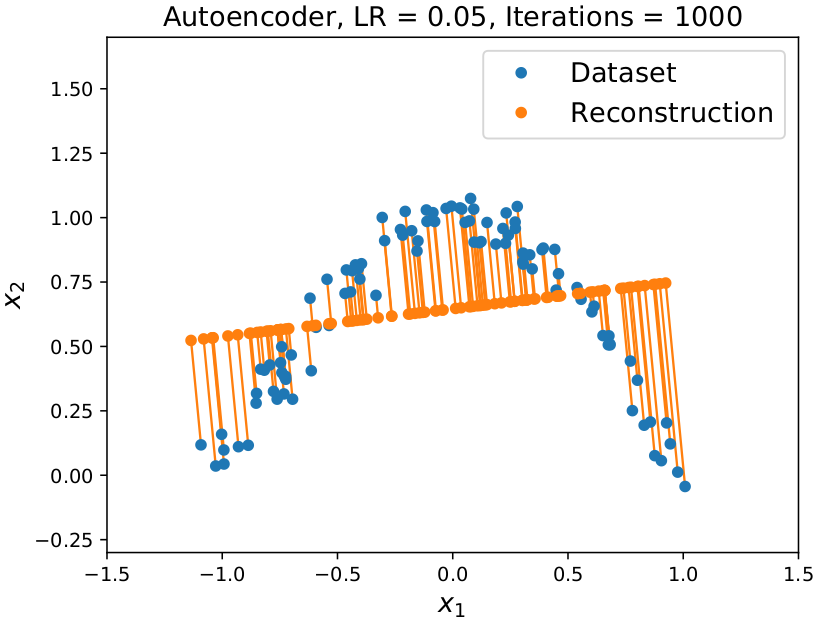
\includegraphics[width=.5\textwidth]{images/s21}
\end{center}
\small{
\begin{itemize}
\item \textbf{Autoencoder reconstruction} with one linear enc/dec layer ($Q=1$)
\end{itemize}
}
\end{frame}


\begin{frame}
  \frametitle{Results on Synthetic 2D Dataset}
\begin{center}
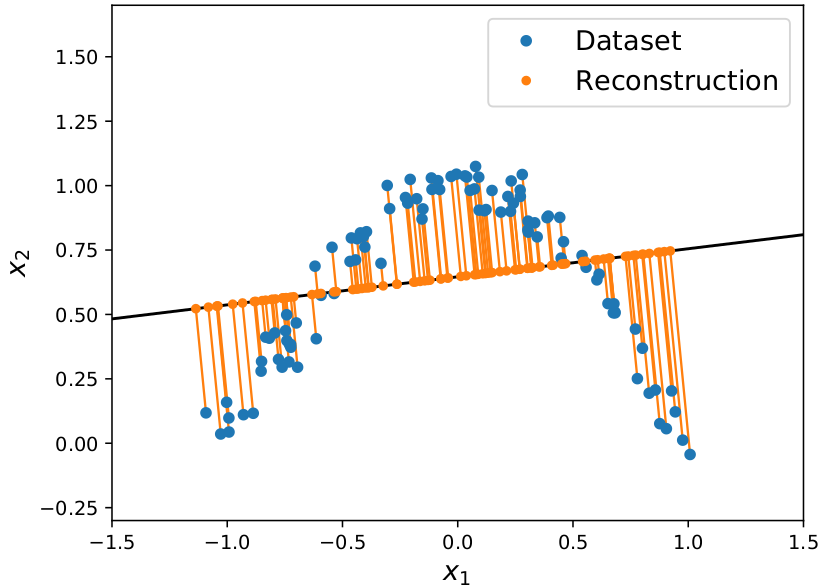
\includegraphics[width=.5\textwidth]{images/s22}
\end{center}
\small{
\begin{itemize}
\item \textbf{PCA reconstructions} on the same dataset with $Q=1$
\end{itemize}
}
\end{frame}

\begin{frame}
  \frametitle{Results on Synthetic 2D Dataset}
\begin{center}
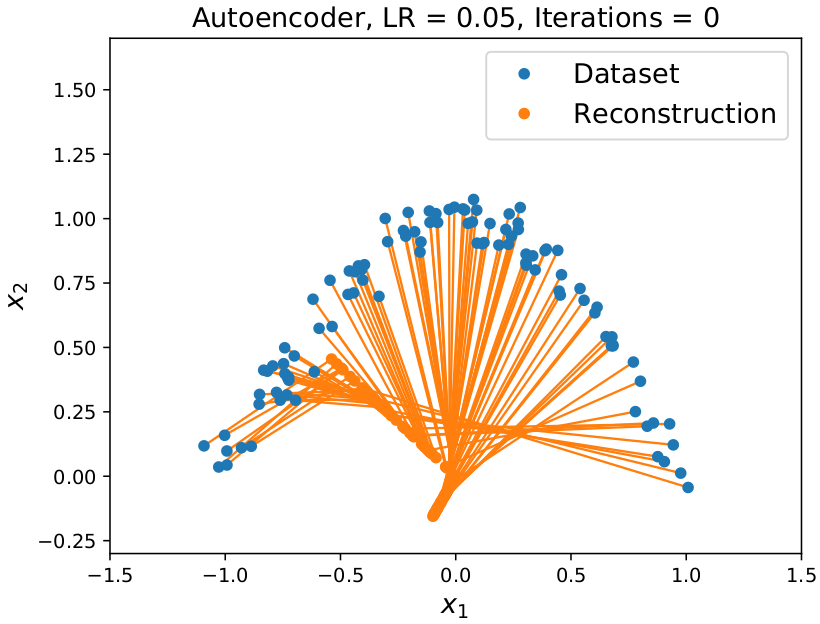
\includegraphics[width=.5\textwidth]{images/s23}
\end{center}
\small{
\begin{itemize}
\item \textbf{Autoencoder reconstruction} with 32D hidden layers ($Q=1$)
\end{itemize}
}
\end{frame}

\begin{frame}
  \frametitle{Results on Synthetic 2D Dataset}
\begin{center}
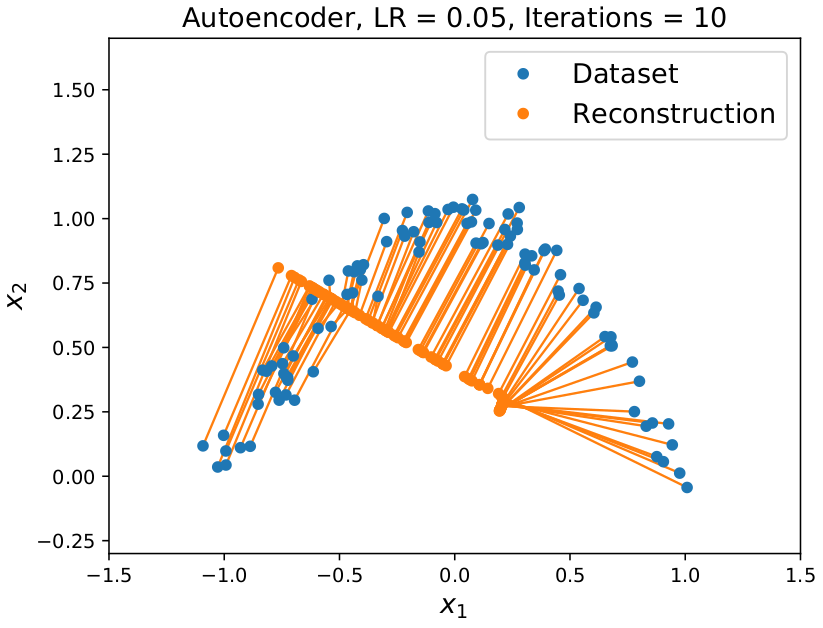
\includegraphics[width=.5\textwidth]{images/s24}
\end{center}
\small{
\begin{itemize}
\item \textbf{Autoencoder reconstruction} with 32D hidden layers ($Q=1$)
\end{itemize}
}
\end{frame}


\begin{frame}
  \frametitle{Results on Synthetic 2D Dataset}
\begin{center}
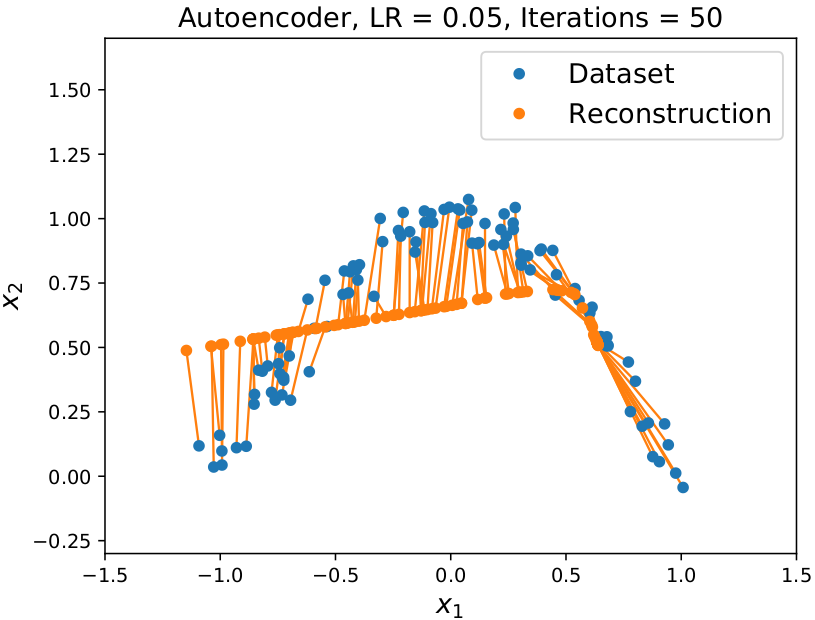
\includegraphics[width=.5\textwidth]{images/s25}
\end{center}
\small{
\begin{itemize}
\item \textbf{Autoencoder reconstruction} with 32D hidden layers ($Q=1$)
\end{itemize}
}
\end{frame}

\begin{frame}
  \frametitle{Results on Synthetic 2D Dataset}
\begin{center}
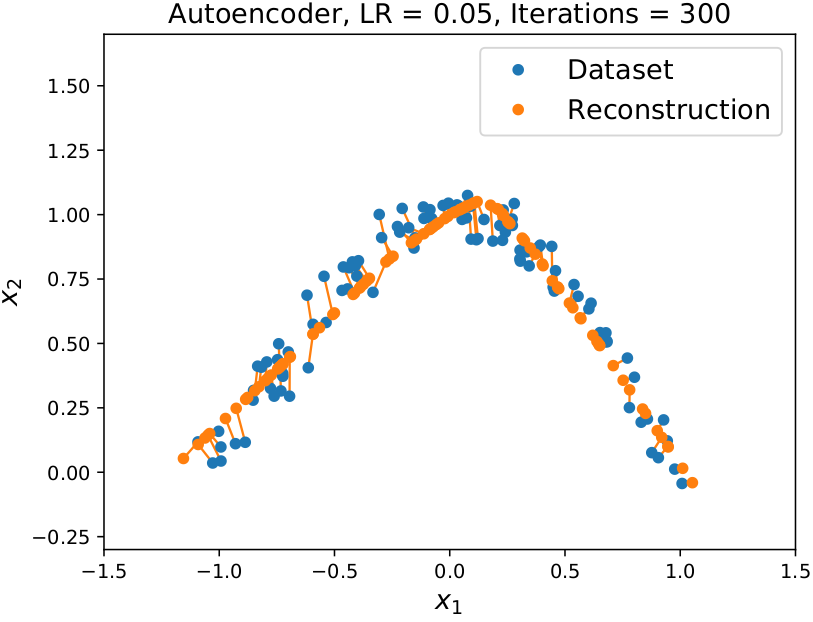
\includegraphics[width=.5\textwidth]{images/s26}
\end{center}
\small{
\begin{itemize}
\item \textbf{Autoencoder reconstruction} with 32D hidden layers ($Q=1$)
\end{itemize}
}
\end{frame}

\begin{frame}
  \frametitle{Results on Synthetic 2D Dataset}
\begin{center}
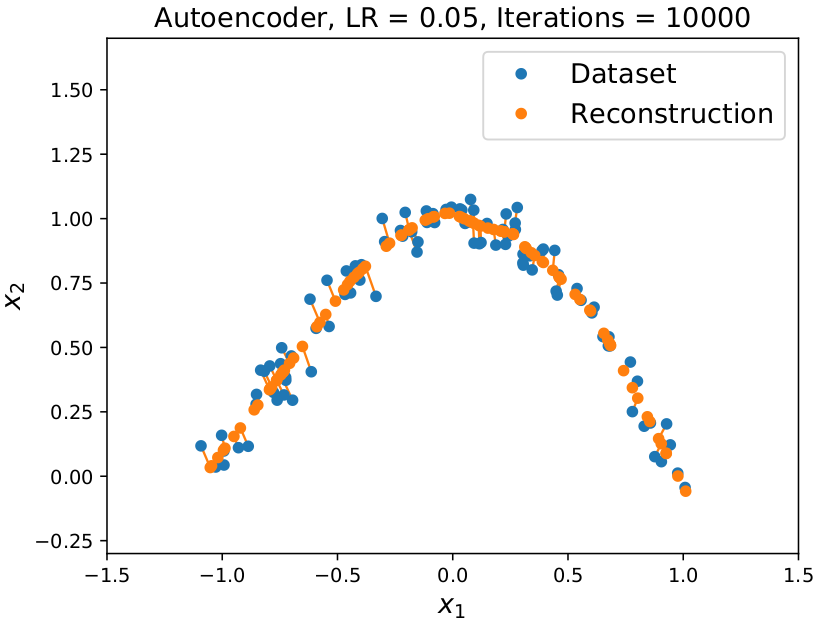
\includegraphics[width=.5\textwidth]{images/s27}
\end{center}
\small{
\begin{itemize}
\item \textbf{Autoencoder reconstruction} with 32D hidden layers ($Q=1$)
\end{itemize}
}
\end{frame}

\begin{frame}
  \frametitle{Results on Synthetic 2D Dataset}
\begin{center}
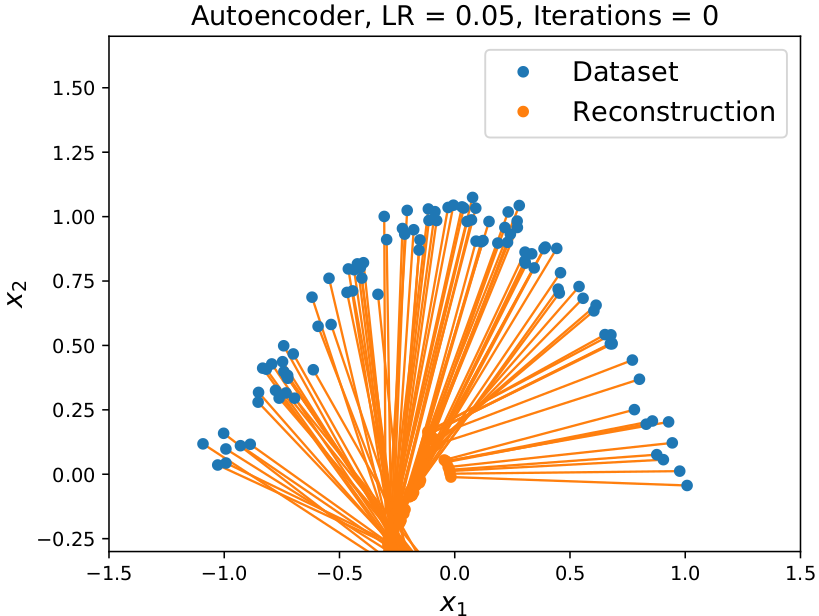
\includegraphics[width=.5\textwidth]{images/s28}
\end{center}
\small{
\begin{itemize}
\item \textbf{Autoencoder reconstruction} with 32D hidden layers ($Q=2$)
\end{itemize}
}
\end{frame}

\begin{frame}
  \frametitle{Results on Synthetic 2D Dataset}
\begin{center}
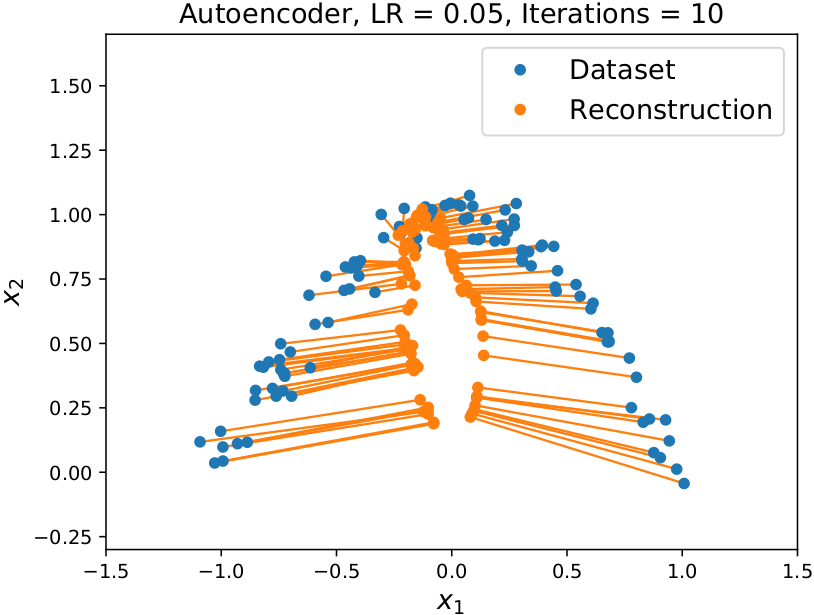
\includegraphics[width=.5\textwidth]{images/s29}
\end{center}
\small{
\begin{itemize}
\item \textbf{Autoencoder reconstruction} with 32D hidden layers ($Q=2$)
\end{itemize}
}
\end{frame}

\begin{frame}
  \frametitle{Results on Synthetic 2D Dataset}
\begin{center}
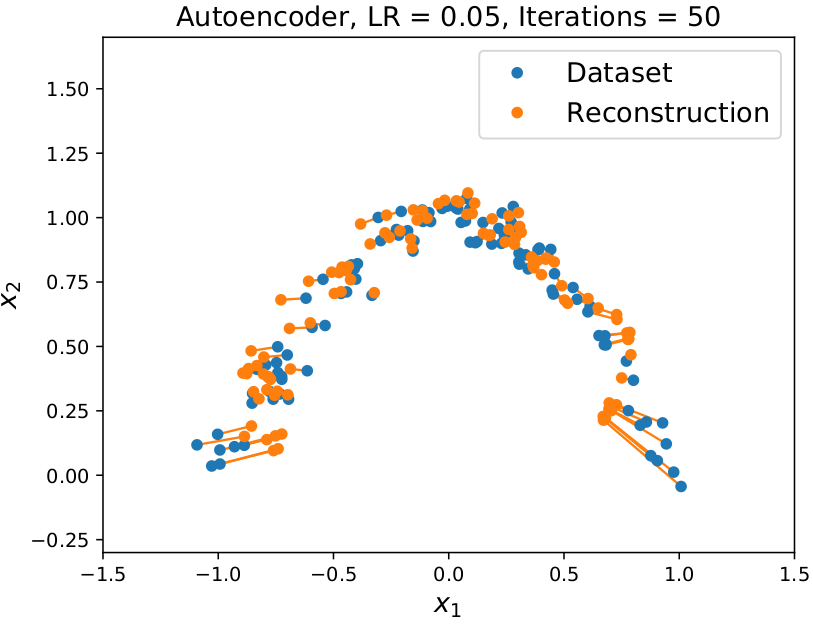
\includegraphics[width=.5\textwidth]{images/s30}
\end{center}
\small{
\begin{itemize}
\item \textbf{Autoencoder reconstruction} with 32D hidden layers ($Q=2$)
\end{itemize}
}
\end{frame}

\begin{frame}
  \frametitle{Results on Synthetic 2D Dataset}
\begin{center}
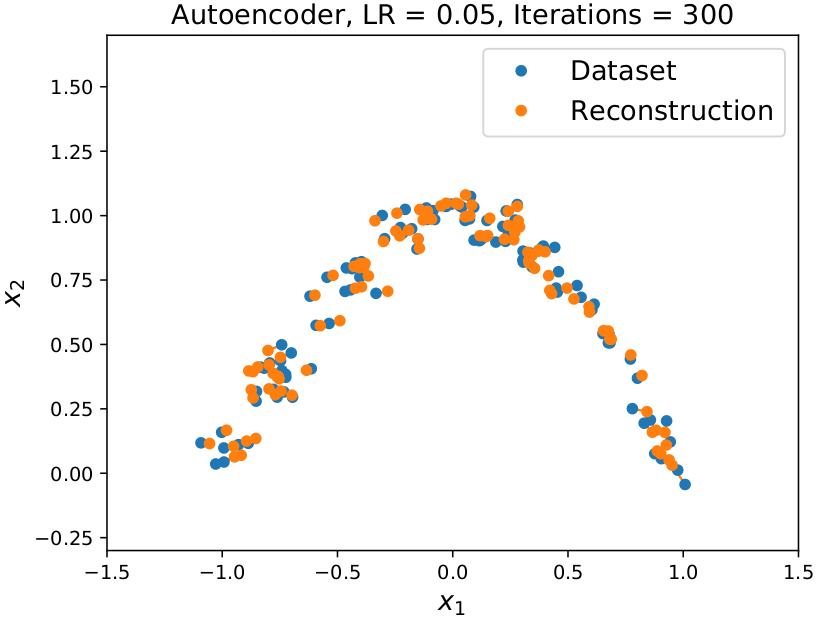
\includegraphics[width=.5\textwidth]{images/s31}
\end{center}
\small{
\begin{itemize}
\item \textbf{Autoencoder reconstruction} with 32D hidden layers ($Q=2$)
\end{itemize}
}
\end{frame}

\begin{frame}
  \frametitle{Results on Synthetic 2D Dataset}
\begin{center}
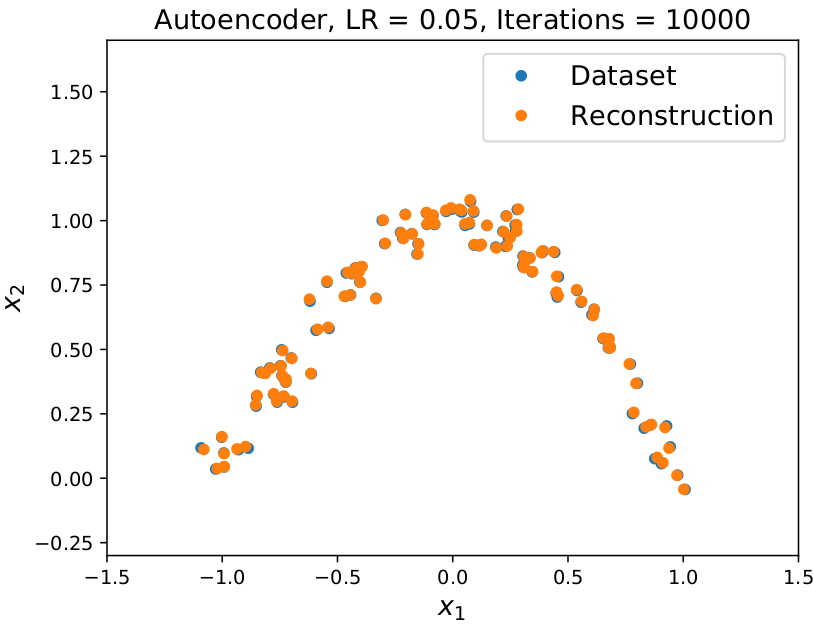
\includegraphics[width=.5\textwidth]{images/s32}
\end{center}
\small{
\begin{itemize}
\item \textbf{Autoencoder reconstruction} with 32D hidden layers ($Q=2$)
\end{itemize}
}
\end{frame}

\begin{frame}
  \frametitle{Comparing Reconstructions}
\begin{center}
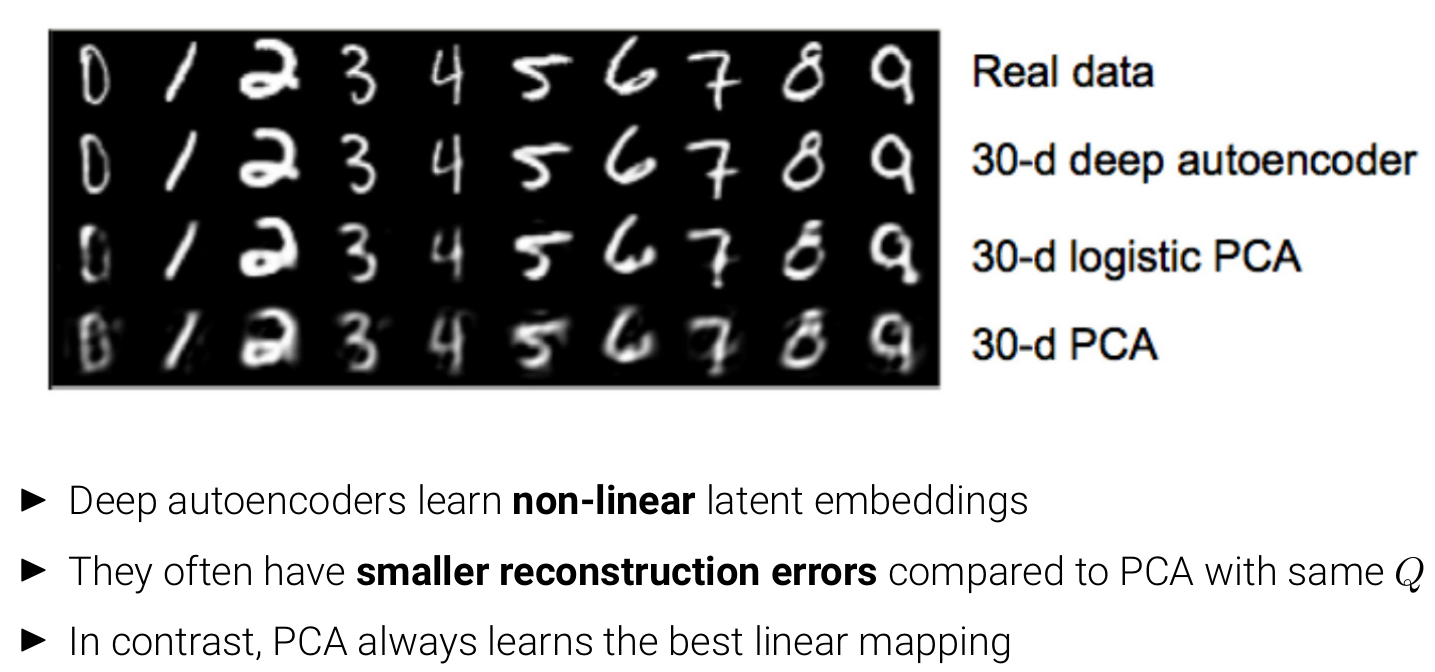
\includegraphics[width=.9\textwidth]{images/s33}
\end{center}
\end{frame}

\begin{frame}
  \frametitle{Denoising Autoencoders}
\begin{center}
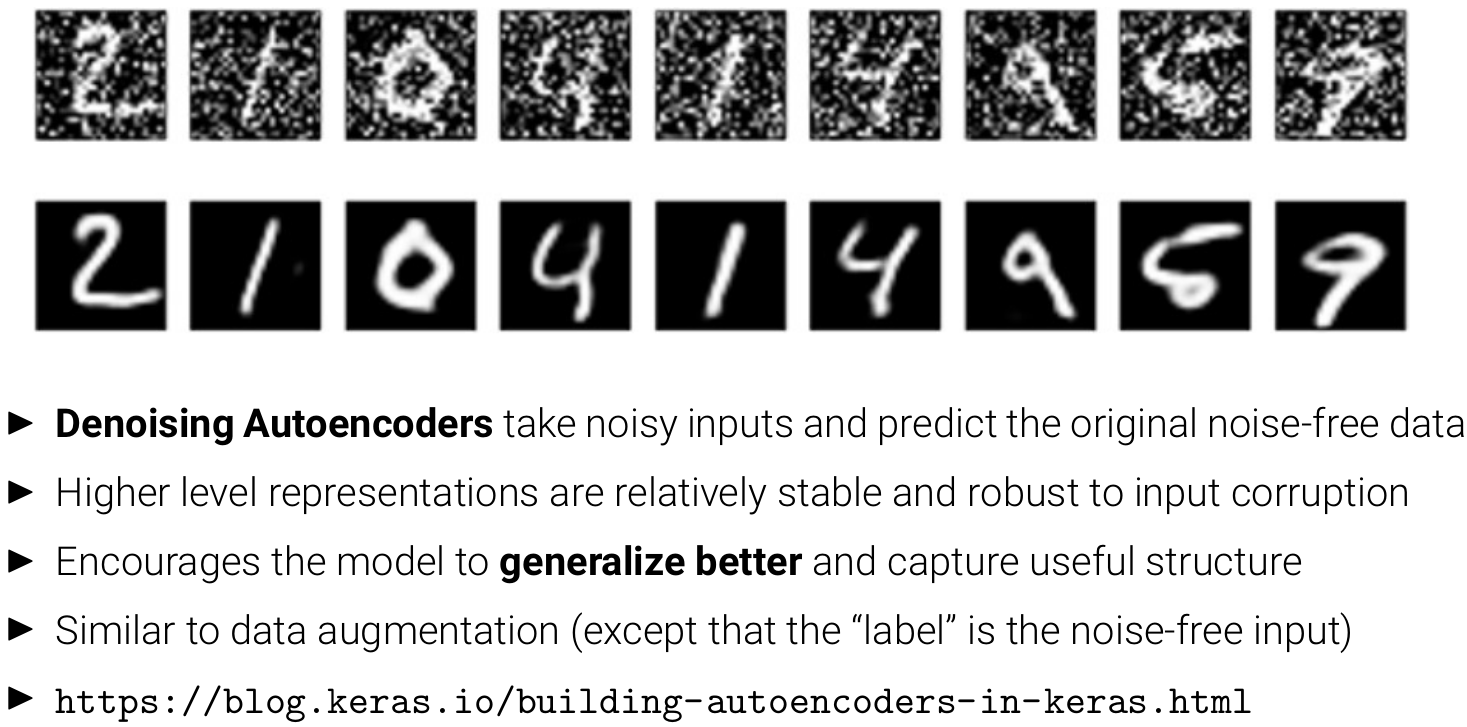
\includegraphics[width=.9\textwidth]{images/s34}
\end{center}
\end{frame}



\begin{frame}
  \frametitle{Variational Autoencoders}
\begin{center}
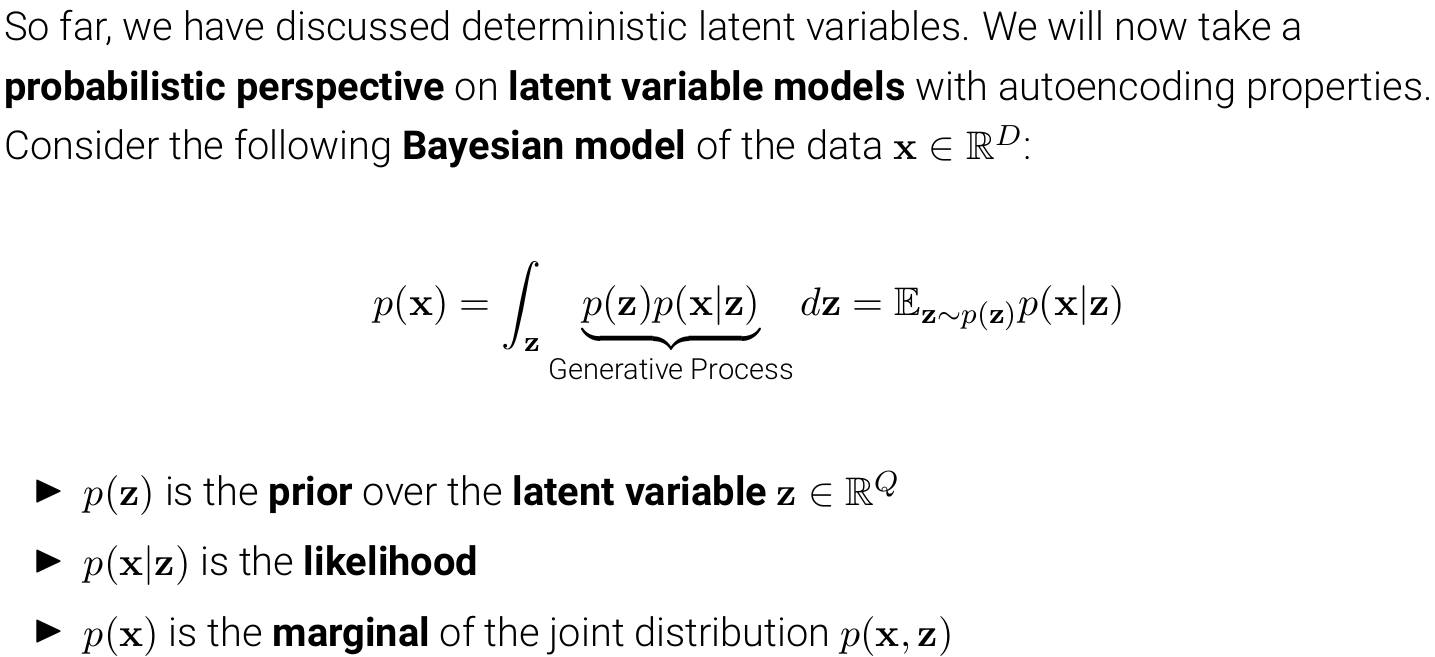
\includegraphics[width=.95\textwidth]{images/s36A}
\end{center}
\end{frame}


\begin{frame}
  \frametitle{Variational Autoencoders}
\small{\textbf{Assumptions:}
\vspace{.4cm}
\begin{itemize}[<+->]
\setlength\itemsep{.8em}
\item The \textbf{prior} model $p(\mathbf{z})$ can be computed and sampled efficiently
\item The \textbf{likelihood} model $p(\mathbf{x}|\mathbf{z})$ is computable
\item We can \textbf{sample} from $p(\mathbf{z})$ and we can compute the proability
of $p(\mathbf{z})$ and $p(\mathbf{x}|\mathbf{z})$ for any given $\mathbf{x}$ and $\mathbf{z}$
\item We will choose \textbf{simple parametric distributions} to achieve this
\end{itemize}
}
%\begin{center}
%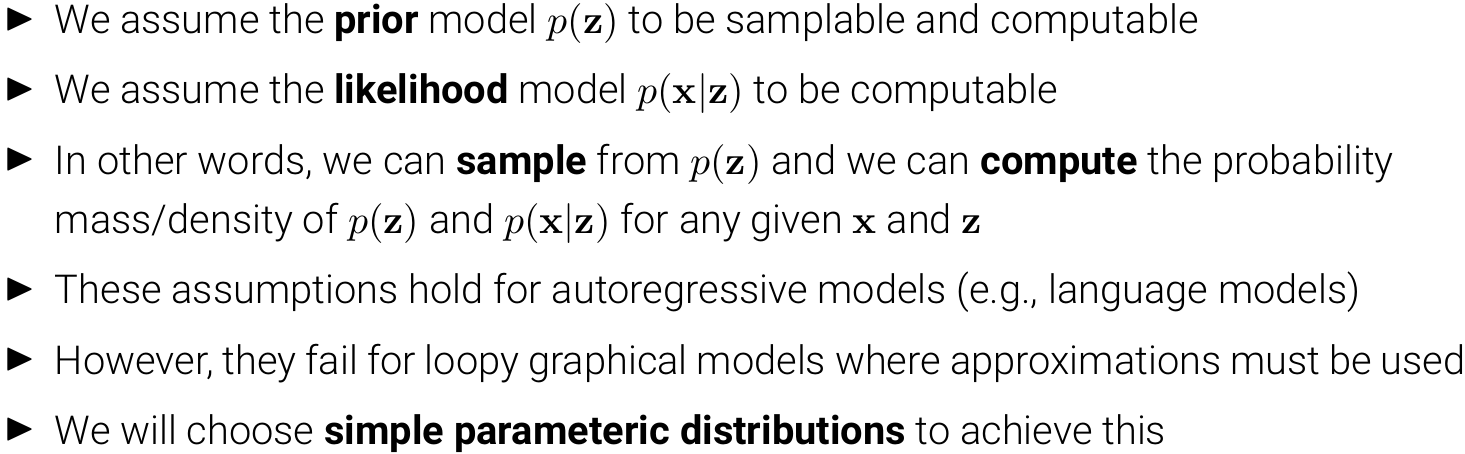
\includegraphics[width=\textwidth]{images/s36}
%\end{center}
\end{frame}



\begin{frame}
  \frametitle{Variational Autoencoders}
\begin{center}
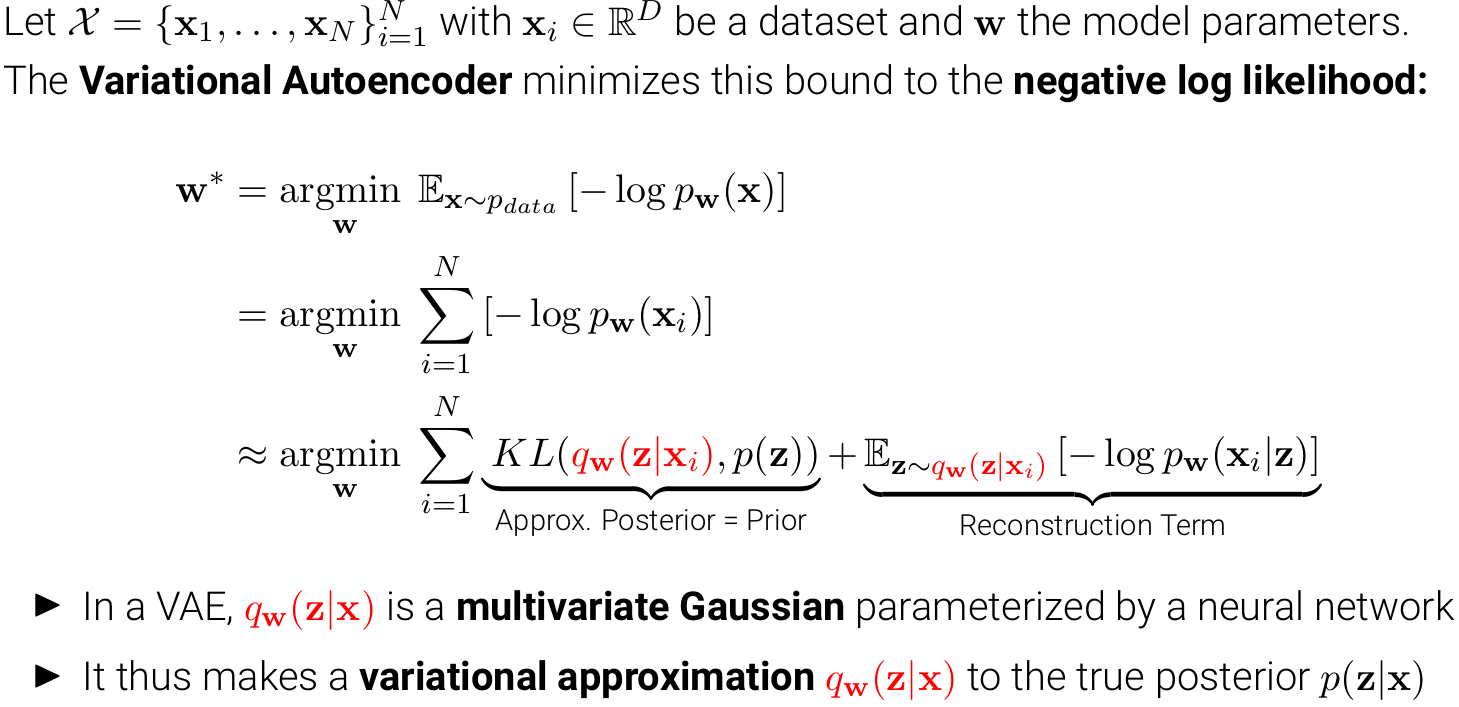
\includegraphics[width=.9\textwidth]{images/s41}
\end{center}
\end{frame}

\begin{frame}
  \frametitle{Variational Autoencoders}
\begin{center}
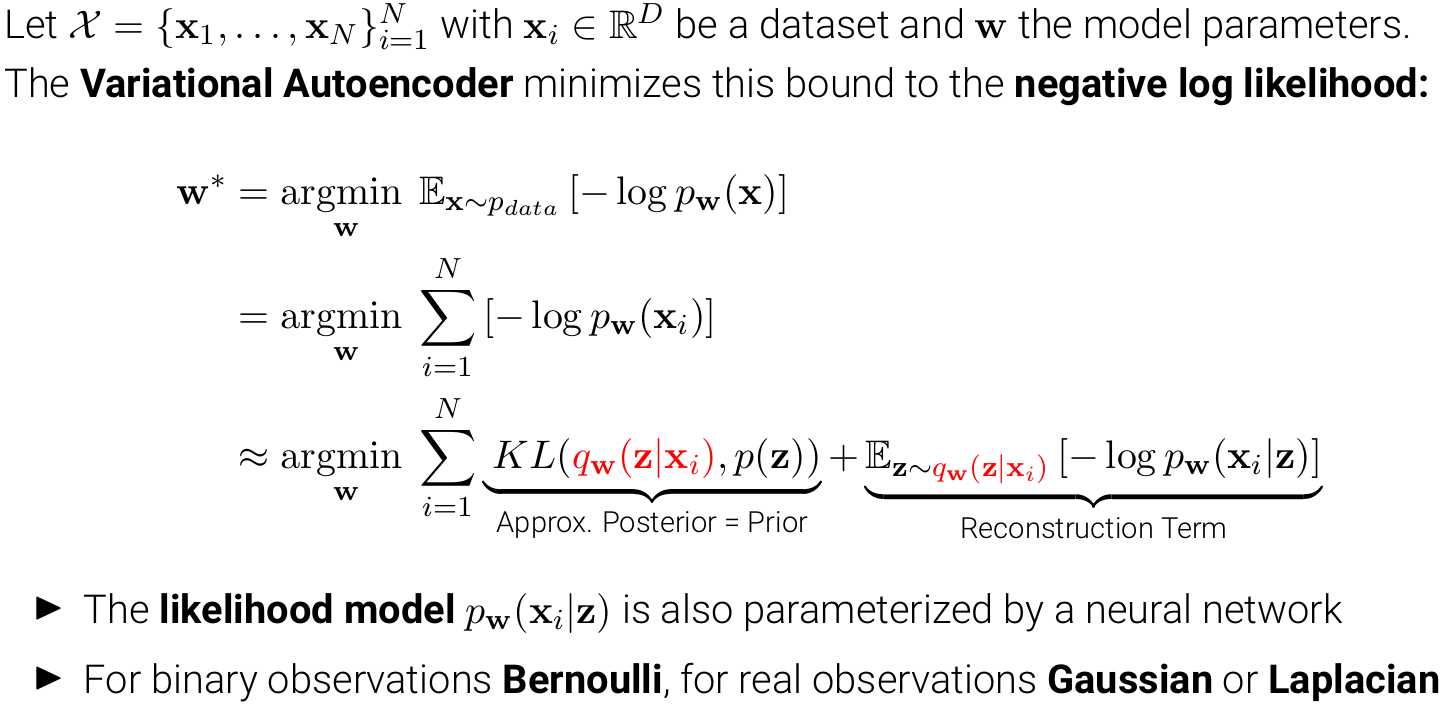
\includegraphics[width=.89\textwidth]{images/s42}
\end{center}
\end{frame}


\begin{frame}
  \frametitle{Learning a VAE}
\begin{center}
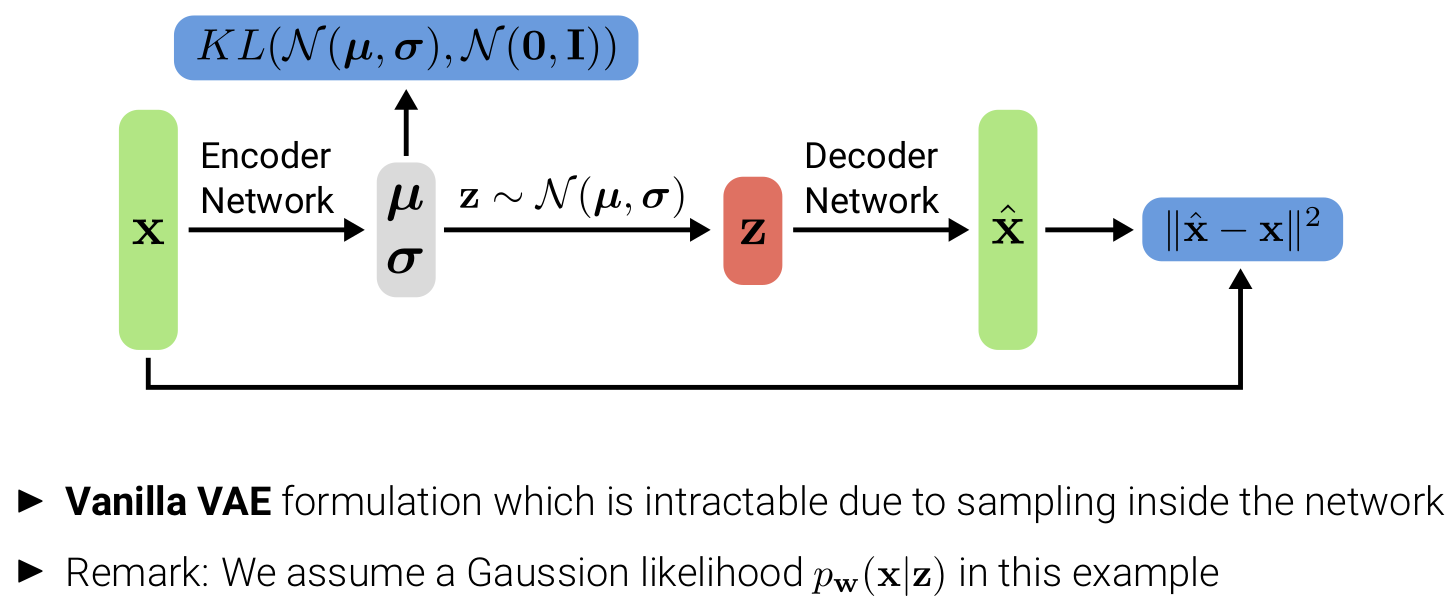
\includegraphics[width=.9\textwidth]{images/s43}
\end{center}
\end{frame}



\begin{frame}
  \frametitle{Learning a VAE}
\begin{center}
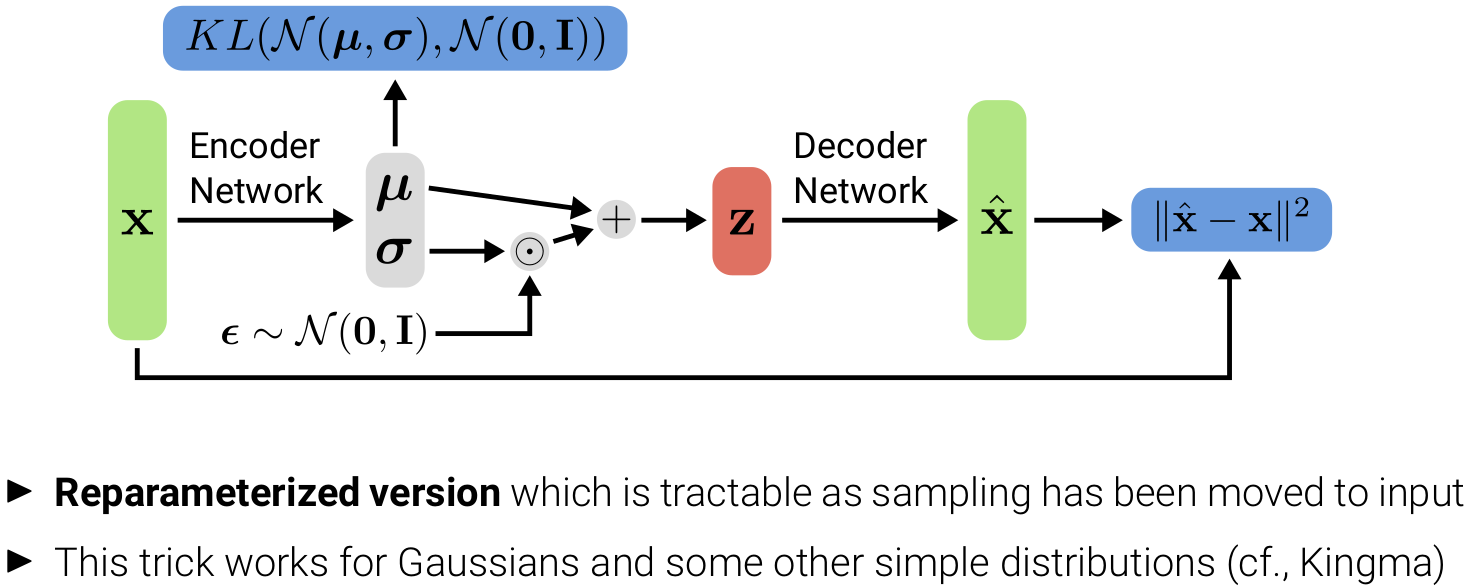
\includegraphics[width=.9\textwidth]{images/s44}
\end{center}
\end{frame}





%\begin{frame}
%  \frametitle{Variational Autoencoders}
%\begin{center}
%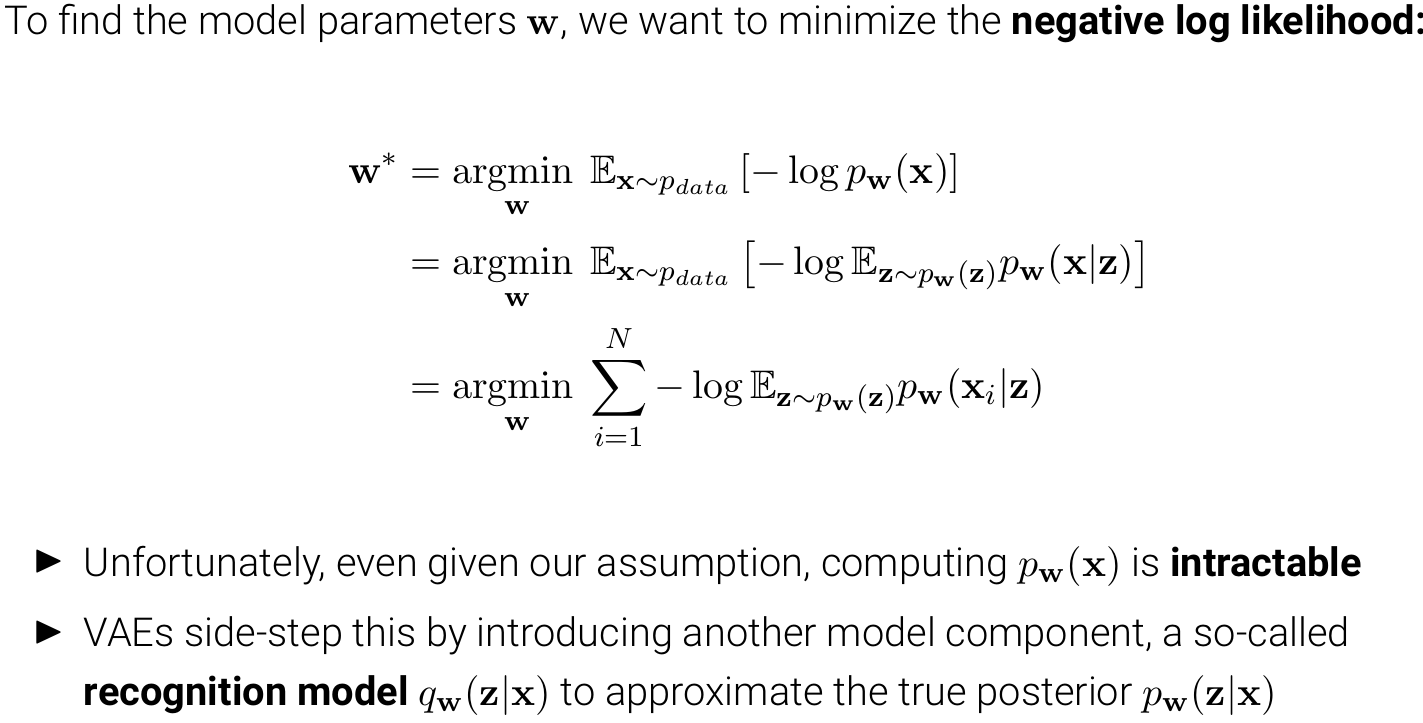
\includegraphics[width=\textwidth]{images/s37}
%\end{center}
%\end{frame}


%\begin{frame}
%  \frametitle{Variational Autoencoders}
%\begin{center}
%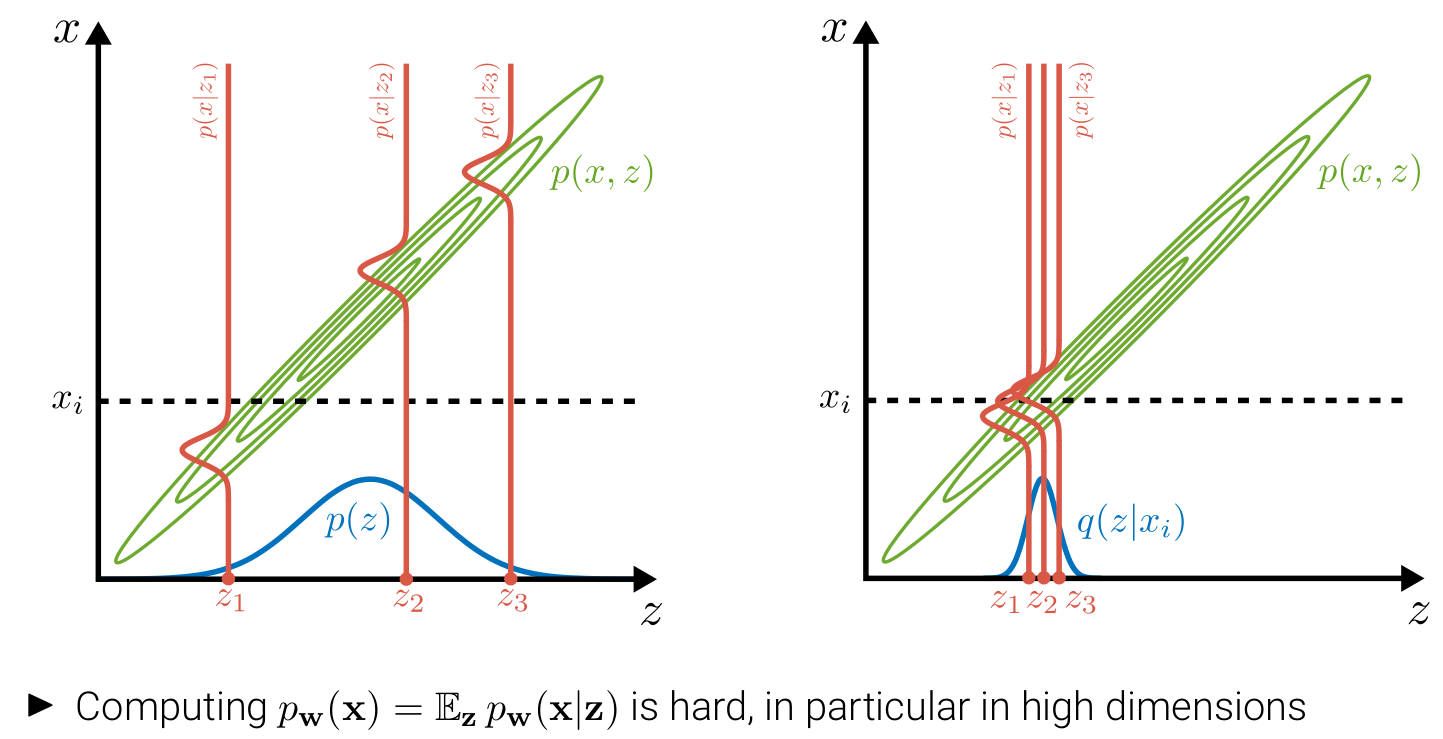
\includegraphics[width=\textwidth]{images/s38}
%\end{center}
%\end{frame}


%\begin{frame}
%  \frametitle{The Evidence Lower Bound (ELBO)}
%\begin{center}
%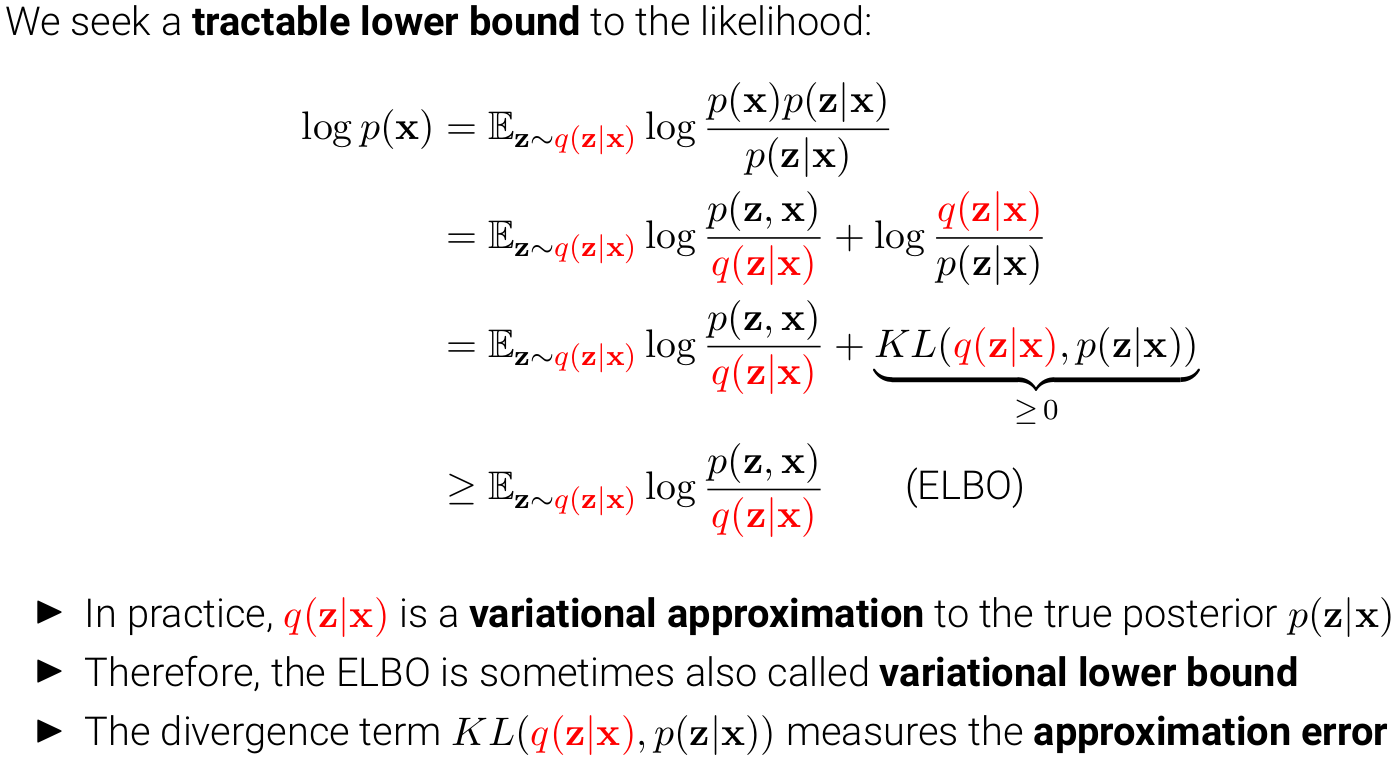
\includegraphics[width=\textwidth]{images/s39}
%\end{center}
%\end{frame}

%\begin{frame}
%  \frametitle{The Evidence Lower Bound (ELBO)}
%\begin{center}
%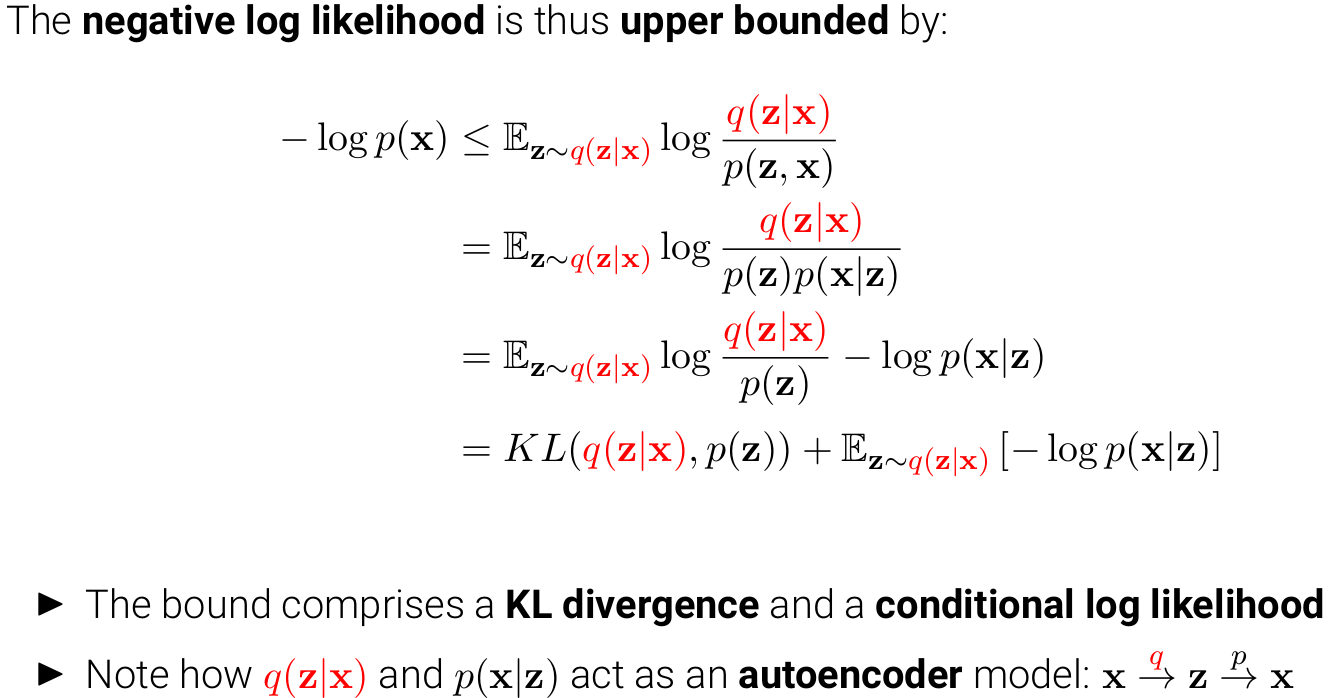
\includegraphics[width=\textwidth]{images/s40}
%\end{center}
%\end{frame}


\begin{frame}
  \frametitle{Example: Natural Image Manifolds}
\begin{center}
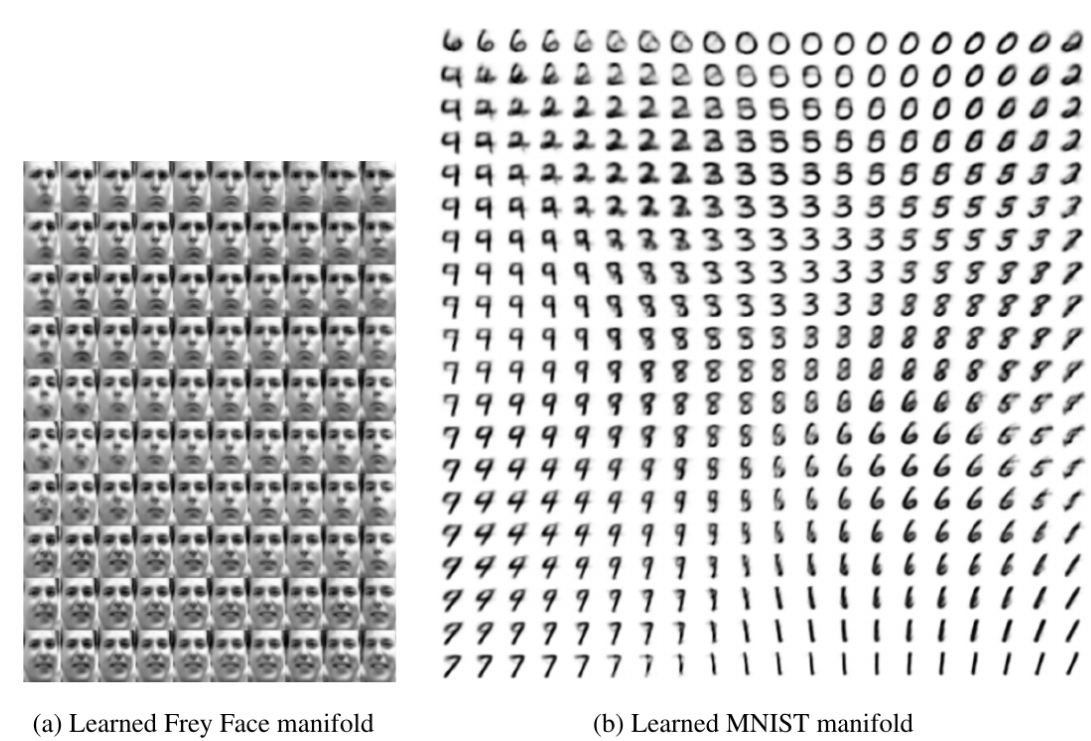
\includegraphics[width=.6\textwidth]{images/s8}
\end{center}
{\scriptsize{
Diederik P. Kingma, Max Welling: Auto-Encoding Variational Bayes. ICLR, 2014.
}}
\end{frame}


\begin{frame}
  \frametitle{Variational Autoencoders (Summary)}
\small{
\begin{itemize}
\item Probabilistic latent variable models
\item Successful in learning useful low-dimensional representations
\item Trained via a bound (ELBO) on the marginal likelihood
\item Sampling from $p(\mathbf{x})$ is straightforward
\item Approximate evaluation of $p(\mathbf{x})$ is possible
\end{itemize}
}
\begin{center}
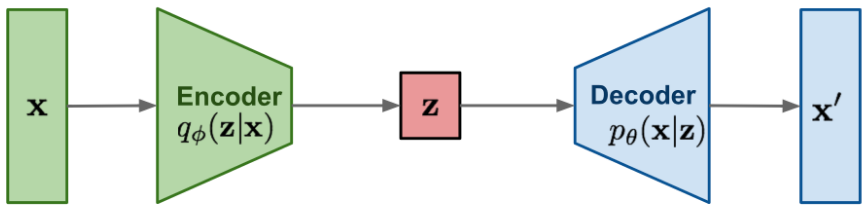
\includegraphics[width=.7\textwidth]{images/vae}
\end{center}
\scriptsize{
Kingma \& Welling Foundations and Trends in Machine Learning: Vol. 12 (2019): No. 4, pp 307-392
}
\end{frame}


\section{Normalizing Flows}

\begin{frame}
  \frametitle{Normalizing flows}
\small{
\textbf{What are normalizing flows?}:
\begin{itemize}
\item A probabilistic latent variable model built on invertible transformations
\item Efficient to sample from $p(\mathbf{x})$
\item Efficient to evaluate $p(\mathbf{x})$
\item Highly expressive
\item Useful latent representation
\item Straightforward to train
\end{itemize}
\vspace{1cm}
Example: Glow model \url{https://openai.com/blog/glow/}
}
\end{frame}



\begin{frame}
  \frametitle{Normalizing flows}
\begin{columns}
\begin{column}{.6\textwidth}

\small{
Basic idea: \textbf{change of variables formula} 
\begin{align*}
p_x(\mathbf{x}) & = p_z( \underbrace{f(\mathbf{x})}_{\text{invertible}})\underbrace{| \det Df(\mathbf{x}) |}_{\text{volume correction}
}\end{align*}
where
\begin{itemize}
\item $\mathbf{z}=f(\mathbf{x})$ with an invertible, differentiable $f(\mathbf{x})$
\item $Df(\mathbf{x})$ is the Jacobian of $f(\mathbf{x})$ \\
(ensures normalization)
\end{itemize}
}
\end{column}
\begin{column}{.4\textwidth}
\begin{center}
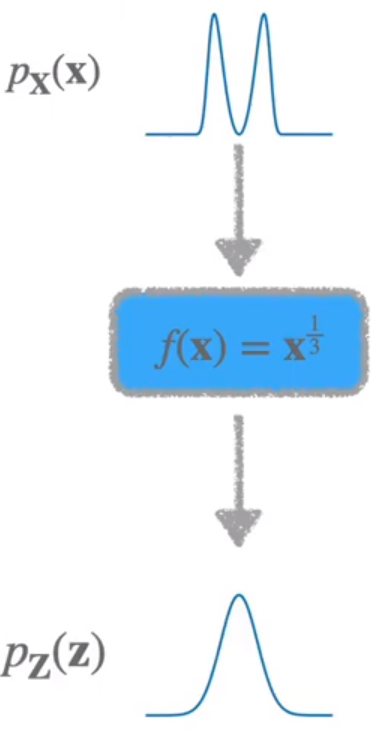
\includegraphics[width=.6\textwidth]{images/inv}
\end{center}
\end{column}
\end{columns}
\end{frame}


\begin{frame}
  \frametitle{Normalizing flows}
\small{
\begin{itemize}
\item
Given $p_x(\mathbf{x})$, fix $p_z(\mathbf{z})$ and find an invertible, differentiable $f(\mathbf{x})$ such that
\end{itemize}
\begin{align*}
p_x(\mathbf{x}) & = p_z(f(\mathbf{x}))|\det Df(\mathbf{x}) |
\end{align*}
}
\begin{center}
\includegraphics[width=\textwidth]{images/flow}
\end{center}
Two pieces:
\begin{itemize}
\item Base measure $p_z(\mathbf{z})$, typically chosen as $\mathcal{N}(\mathbf{0},\mathbf{I})$
\item Flow $f(\mathbf{x})$ must be invertible and differentiable
\end{itemize}
\end{frame}

\begin{frame}
  \frametitle{Normalizing flows}
\begin{columns}
\begin{column}{.7\textwidth}
\small{
Training via maximum (log-)likelihood
\begin{align*}
\max_\theta \sum_{i=1}^N \log p_z( f(\mathbf{x}_i ; \theta) ) + \log | \det Df(\mathbf{x}_i;\theta) |
\end{align*}
where $\theta$ are the parameters of the flow $f(\mathbf{x}_i;\theta)$
\vspace{.5cm}

If learned properly:
\begin{itemize}
\item Exact density evaluation: $p_x(\mathbf{x})  = p_z( f(\mathbf{x}))| \det Df(\mathbf{x}) |$
\item Sampling
\begin{itemize}
\item Sample $\mathbf{z}\sim \mathcal{N}(\mathbf{0},\mathbf{I})$
\item Compute $\mathbf{x} = f^{-1}(\mathbf{z})$
\end{itemize}
\end{itemize}
}
\end{column}
\begin{column}{.3\textwidth}
\begin{center}
\includegraphics[width=.7\textwidth]{images/yeah}
\end{center}
\end{column}
\end{columns}
\end{frame}

\begin{frame}
  \frametitle{Normalizing flows}
\small{
\begin{itemize}[<+->]
\item \textbf{Main challenge:} Design an invertible and differentiable flow that is also
\begin{itemize}
\item Sufficiently expressive
\item Efficient computation of inverse and Jacobian determinant
\end{itemize}
\item Key idea: Compositions of simpler flows
\end{itemize}
}
\visible<5->{
\begin{center}
\includegraphics[width=.8\textwidth]{images/inversions}
\end{center}
}
\end{frame}

\begin{frame}
  \frametitle{Normalizing flows}
\small{
\begin{itemize}[<+->]
\item The determinant of the Jacobian factorizes 
$$\det Df=\det \prod_{k=1}^K Df_k=\prod_{k=1}^K \det Df_k$$
\end{itemize}
}
\end{frame}


\end{document}
